% CREATED BY DAVID FRISK, 2015
\chapter{Theory}

In the following sections, examples of a figure, an equation, a table, a chemical structure, a list, a listing and a to-do note are shown.

\section{Structural theory of masonry structures}

Masonry is a composition or assemblage of building elements. The most common types of these elements are stones and bricks. It can though be in any shape it can be done with or without mortar but the structural action is similar. According to Heyman it is wise to and convenient to regard a masonry building as a collection of dry stones or bricks that are placed on one another to to form a stable structure. The mortar cannot be accounted since it may have reduced its structural influence with time - it cannot be assumed to add strength to the construction. The stability of the structure relies on the compaction under the gravity of its components. "A general state of compressive stress exists, but only feeble tensions can be resisted."\\

\subsection{Structural design}
Speaking in terms of general design there are three main structural criterion's, those of \textit{strength, stiffness and stability}. The first implies that the material should resist the internal stresses and the second ensures not to high deflections. These criterion's are not the crucial regarding masonry structures, it is the stability that is of most concern.\\

Heyman uses an masonry arch to illustrate this. The load applied on the load is it self-weight and an external point load. The stresses are low and the deflection negligible until a certain magnitude of the point load is reached and it collapses. The stresses are still low in the structure but the internal forces cannot be held inside the geometry of the arch. This leads to the formation of four frictionless hinges that turns the structure into a collapse mechanism.\\   

\begin{figure}[H] 
\centering
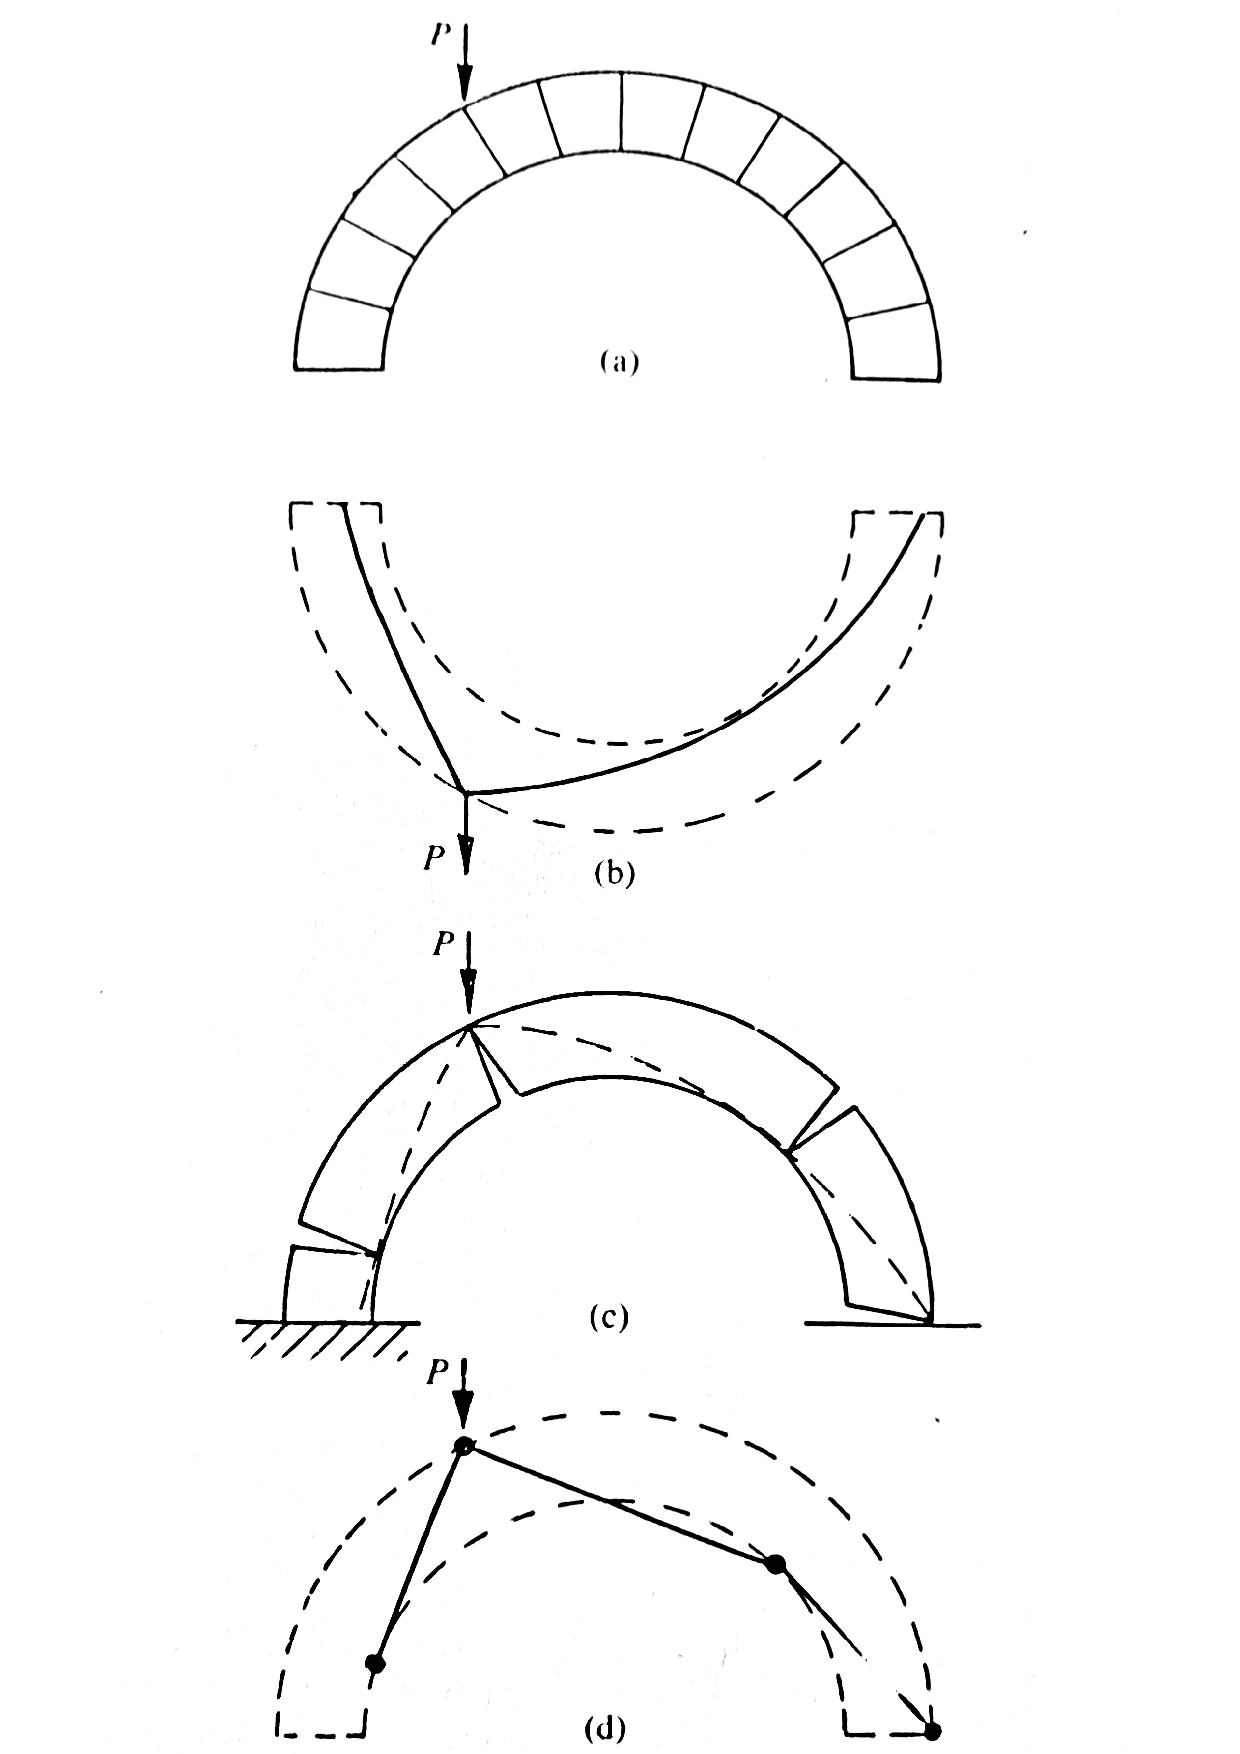
\includegraphics[width=0.5\linewidth ]{figure/Theory/heyman3.pdf}
\caption{Collapse mechanism of masonry vault by an asymmetric load}
\label{fig:arch2}
\end{figure}

Heyman imposes a method of based on plastic analysis for the structural design of masonry rather than the elastic analysis. One reason is that an elastic solution might not be possible, an arch consisting of rigid blocks will not deform themselves and will therefore not obey the rules of elastic analysis. Another reason is that there are uncertainties regarding the structure and how the boundary conditions change during time. Therefore an elastic analysis might change dramatically with time. The so-called plastic designer knows that the there are infinite ways to achieve equilibrium and that the solution he has found is just one of them. The plastic designer takes this into account and applies the theorems of plasticity to ensure that the structure will not fail. \\


\begin{itemize}
\item The lower bound, or safe theorem
\item The upper bound, or unsafe theorem
\item The uniqueness theorem
\end{itemize}

This will be described more in detail later. Important to understand that the hinges formed are natural behaviour of the masonry structures, in a similar way as the reinforced concrete is suppose to crack otherwise the reinforcement is unnecessary. So the designer should be aware of the of this phenomena. A sufficient hinges, or cracks, are fine but for instance the arch will collapse when four of these have formed. This can of course easily be very complicated to read in more complex structures where many different elements interact.

\begin{figure}[H] 
\centering
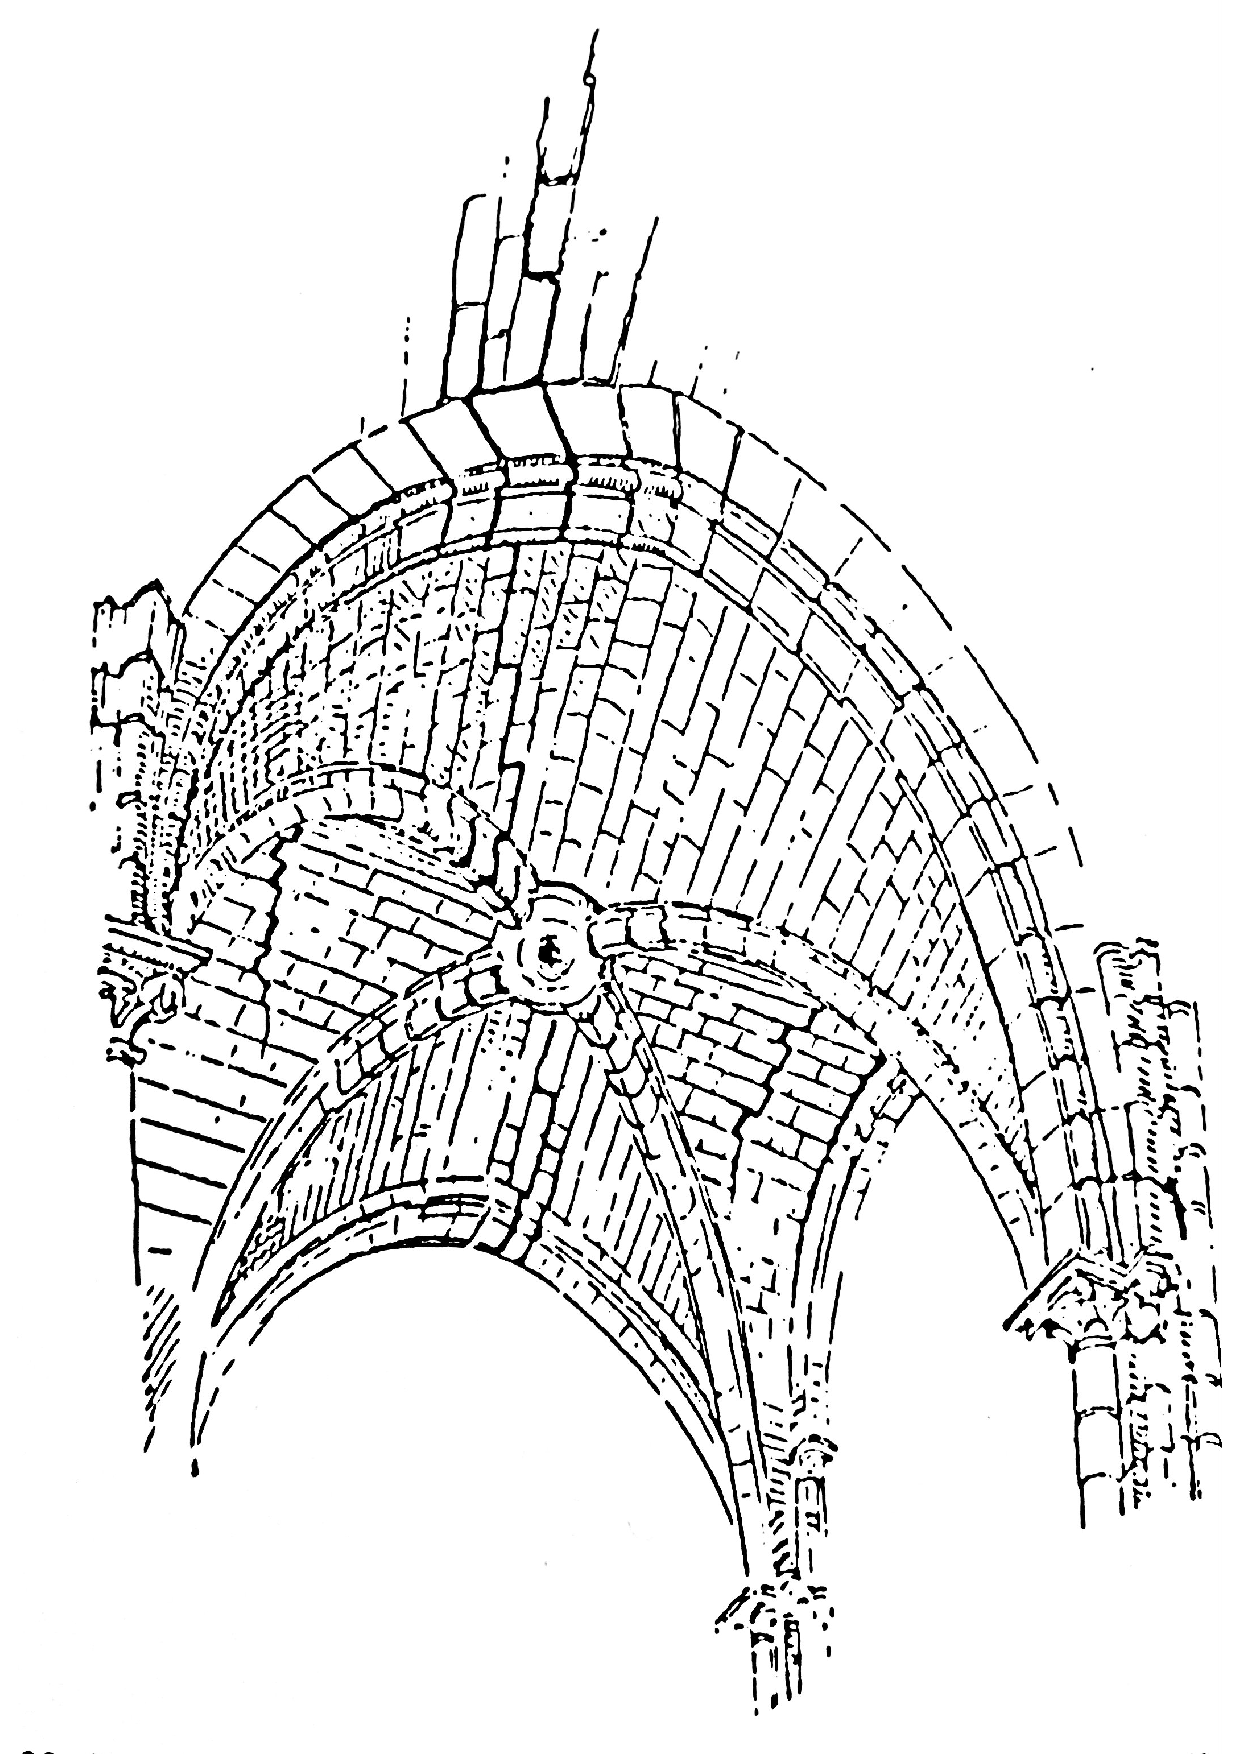
\includegraphics[width=0.5\linewidth ]{figure/Theory/cracksHeyman.pdf}
\caption{Collapse mechanism of masonry vault by an asymmetric load}
\end{figure}

\subsection{Limit Design Principles}

The limit design principles Heyman purposes for masonry is similar to the ones used is similar to the plastic hinge theory used for plastic design of steel frames. This implies that hinges formed causes the structure to become a mechanism. To be able to apply the same theory and theorems for masonry structures Heyman makes three assumptions for the properties of the material:\\



\textit{"(i) Stone has no tensile strength. This assumption is almost exactly true if a structure,
like an arch, is under consideration, made up of voussoirs laid either dry or with very
weak mortar. Although the stone itself may in fact have some tensile strength, the joints
will not, and no tensile forces can be transmitted from one portion of the structure to
another. The assumption of no tensile strength is, in accordance both with common sense
and with the corollaries of the general principles established below, a safe assumption.
It may be slightly too safe if the stone structure is not of the voussoir type, and if tensile
forces can be transmitted by the interlocking of perhaps randomly oriented stones.}

\textit{(ii) The general stress levels are so low that, for the purposes of calculation, the compressive
strength of stone is effectively infinite. This is a slightly unsafe assumption, and
will be discussed more fully later.}

\textit{(iii) Sliding of one stone upon another cannot occur. This seems a reasonable assumption
(it did to Coulomb, as noted above). It implies that wherever there is a weak plane, for
example between voussoirs, the line of thrust should not depart too far from normality
to that plane. (The collapse of Beauvais may have been initiated by sliding.)" }Stone Skeleton 660

The hinges are formed when, as shown in figure \ref{fig:arch2}, when the line of thrust cannot contain itself inside the geometry. A thrust that follows the centre line of the structure results in pure axial forces, and when moving outside it results in a minor moment that until a certain point that will be negligible due to the compression of the self weight.

\begin{figure}[H]
\centering
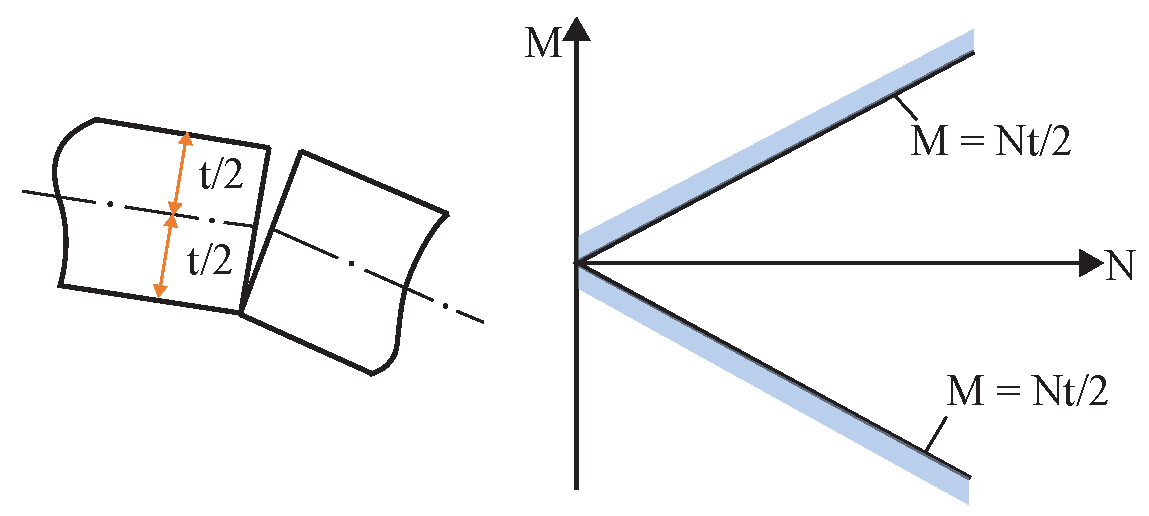
\includegraphics[width=0.9\linewidth ]{figure/Theory/Plasticity.pdf}
\caption{Limit condition for masonry voussoirs}
\end{figure}

This represents a block of infinite stress capacity since a normal stone or brick would crush when the contact area gets to small. Therefore there are some safety factors that need to be applied.


\subsubsection{Safety factor}

\begin{figure}[H]
\centering
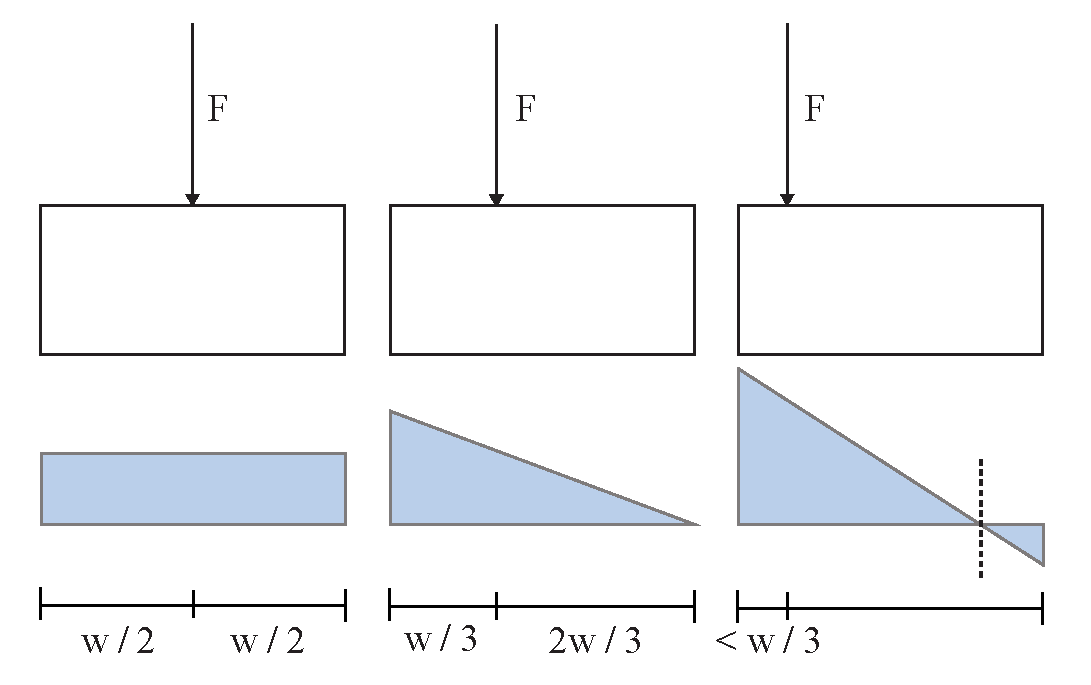
\includegraphics[width=0.9\linewidth ]{figure/Theory/Safety.pdf}
\caption{This shows the middle third rule applied to a block. redrawn from Block...}
\end{figure}


\subsection{Plasticty theorems}
\subsubsection{Lower Bound Theory}


If a distribution of moments can be found which satisfies the above equilibrium and yield conditions the structure is either safe or just on the point of collapse.
\subsubsection{Upper Bound Theory}


If a loading is found which causes a collapse mechanism to form then the loading must be equal to or greater than the actual collapse load.

Generally, in plastic analysis, the upper bound theorem is used. Possible collapse mechanisms are formulated and the corresponding collapse loads calculated. From the upper bound theorem we know that all mechanisms must give a value of collapse load which is greater than or equal to the true collapse load so that the critical mechanism is the one giving the lowest load. It is possible that a mechanism, which would give a lower value of collapse load, has been missed. A check must therefore be carried out by applying the lower bound theorem.


\subsubsection{The uniqueness theorem}
"The uniqueness theorem may be stated for masonry as follows: If a line of thrust can be found which represents an equilibrium state for the structure under the action of the given external loads, which lies wholly within the masonry, and which allows the formation of sufficient hinges to transform the structure into a mechanism, then the structure is on the point of collapse; further, if the loads can all be specified as ratios of one of their number (proportional loading), and the loads have been notionally increased from their working values to the collapse values by a load factor, then the value of that load factor at collapse is unique. "


\section{Tensor Analysis}

Britannia
"Tensor analysis, branch of mathematics concerned with relations or laws that remain valid regardless of the system of coordinates used to specify the quantities. Such relations are called covariant. Tensors were invented as an extension of vectors to formalize the manipulation of geometric entities arising in the study of mathematical manifolds."

\subsection{Index notation}
The index notation simplifies writing quantities as well as equations. In the index notation there are two types of indices, \textit{free indices} and \textit{summation indices}.\\

\textit{Free indices} are those who are used only once per quantity. If you have a Cartesian coordinate system the integer will take values 1,2 and 3. It is possible to use several free indices.

\begin{align*} 
    a_\alpha  &\Leftrightarrow a_1 , a_2, a_3 \\ 
   a_{\alpha \beta}  &\Leftrightarrow a_{11},a_{12},a_{13},a_{21},a_{22},a_{23},a_{31},a_{32},a_{33}
\end{align*}

\textit{Summation indices} are used twice per quantity and indicates a  summation of that index. Using Cartesian coordinates it will range from 1 to 3.
\begin{align*} 
    a_{\alpha \alpha}  &\Leftrightarrow \sum\limits_{\alpha=1}^3  a_{\alpha \alpha} \\ 
   a_{\alpha}b_\alpha  &\Leftrightarrow \sum\limits_{\alpha=1}^3  a_{\alpha}b_\alpha 
\end{align*}

\subsection{2nd order Tensors}
2nd order tensors are physical quantites that describe how vectors change with e.g direction and position in space. A 2nd order tensor \textbf{T} is represented in a orthonomal coordinate system $\{\hat{\textbf{e}_1},\hat{\textbf{e}_2} , \hat{\textbf{e}_3}\}$ as

\begin{equation}
\textbf{T} = T_{\alpha\beta}\hat{\textbf{e}_\alpha},\hat{\textbf{e}_\beta}
\end{equation}


%\section{Geometry}
\section{Differential Geometry}

Differential geometry is a mathematical discipline that uses the techniques of differential calculus, integral calculus, linear algebra and multilinear algebra to study problems in geometry. The theory of plane and space curves and surfaces in the three-dimensional Euclidean space formed the basis for development of differential geometry during the 18th century and the 19th century. (Wikipedia)

Something that is dependent on Smooth geometry and functions. That is because it is called Differential geometry... etec etec 


\newcommand{\upperRomannumeral}[1]{\uppercase\expandafter{\romannumeral#1}}
\newcommand{\lowerromannumeral}[1]{\romannumeral#1\relax}


\subsection{Intrinsic and Extrinsic properties}

Declare the difference of embodied properties and those dependent on how you define things etc etc

\begin{figure}[H]
\centering
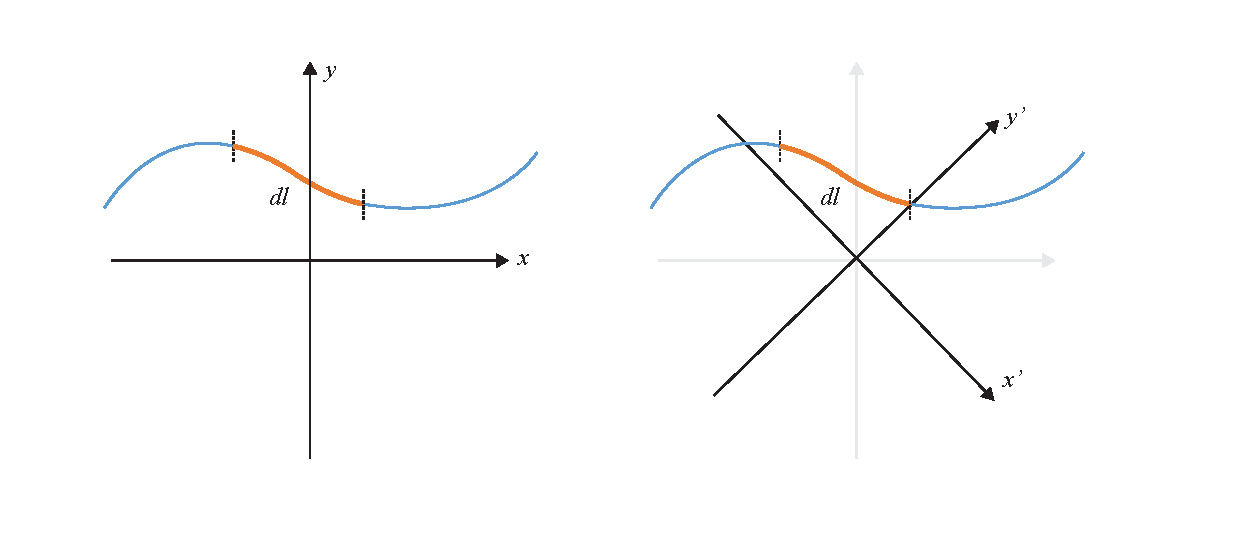
\includegraphics[width=0.9\linewidth ]{figure/Theory/intrisic_extrinsic2.pdf}
\caption{The length of the curve is the same regardless of coordinate system.}
\end{figure}


\begin{figure}[H]
\centering
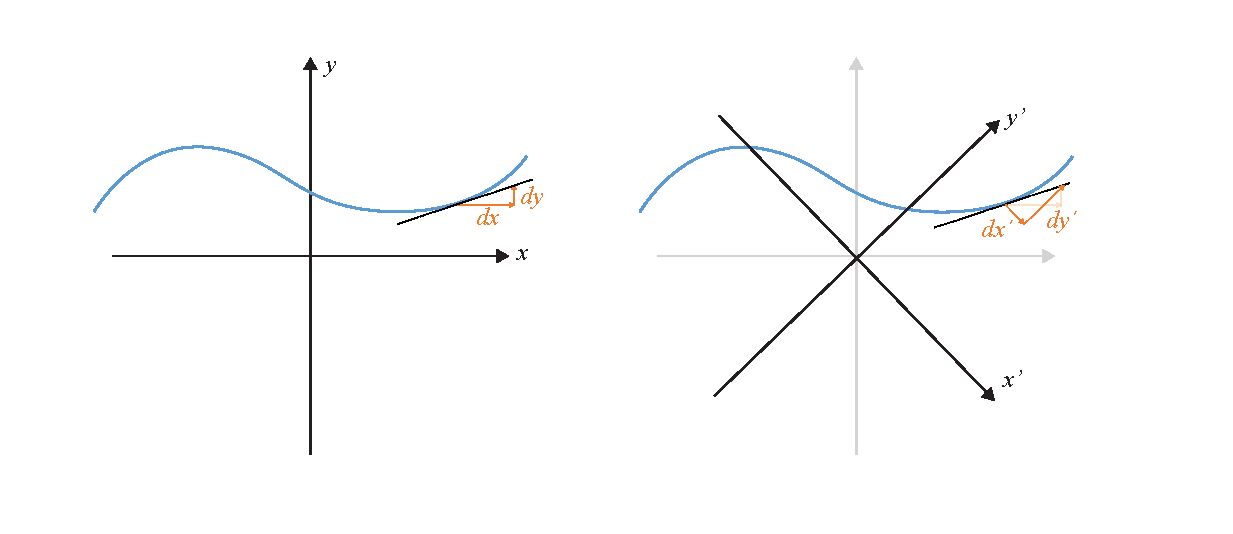
\includegraphics[width=0.9\linewidth ]{figure/Theory/intrisic_extrinsic1.pdf}
\caption{The tangent differs depending of which direction you refer to. }
\end{figure}

\subsection{Curves In Space}
There are many examples of Curves and most of you have used various of them. Common examples might be a line, a parabola or a circle. 


\begin{figure}[H]
\centering
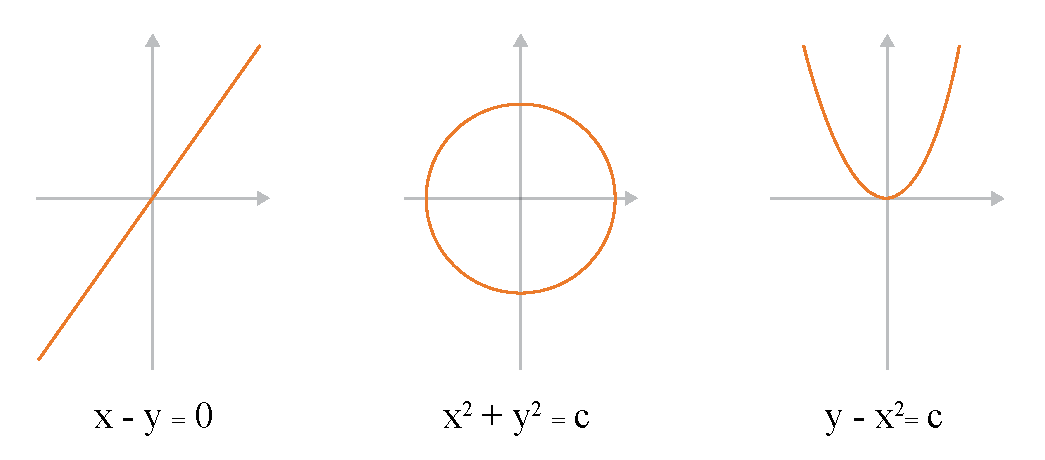
\includegraphics[width=0.9\linewidth ]{figure/Theory/CurveExample.pdf}  \caption{Example of Curves, Presley }
\end{figure}

Using this notation means that you describe them in a Cartesian equation $f(x,y) = c$
Where $f$ is a function of $x$ and $y$ and $c$ is a constant.From this point of view we see a curve as a set of points namely

$$ \mathcal{C}\quad =\quad \left\{ (x,y) \in \mathbb{R}^2\quad |\quad f(x,y) = c \right\} $$


It is sometimes more efficient to describe curves in another way, as a parametrized curve. Where the curve is described by a function $\gamma$ of a scalar parameter $t$ with vector values(in $\mathbb{R}^2$ for a plane curve, in $\mathbb{R}^3$ for a curve in space). 

\begin{equation}
\gamma(t) = x(t)\textbf{i} +  y(t)\textbf{j}+  z(t)\textbf{k},\quad in\quad \mathbb{R}^3
\end{equation}

A proper definition of a parametrized curve can be read in Presley.

\vspace{5mm} %5mm vertical space

A \textit{parametrized curve} in $\mathbb{R}^n$ is a map $\gamma : (\alpha,\beta) \rightarrow \mathbb{R}^n $, for some $\alpha,\beta$ with $-\infty\leqslant\alpha<\beta\leqslant\infty$ 

The symbol $(\alpha,\beta)$ denotes the open interval $(\alpha,\beta) = {t\in \mathbb{R} | \alpha < t < \beta}$

\vspace{5mm} %5mm vertical space

To give an example when this is useful we can take the circle which can be described as $x^2+y^2=1$. A common choice to parametrize is to choose $x = cos(t)$ and $y = sin(t)$ which clearly holds the initial statement $cos(t)^2 + sin(t)^2 = 1$.  

Written in parametric form $\gamma(t) = (cos(t),sin(t))$. A useful property of this parametrization is that we can differentiate this expression infinitely many times. This is very useful when computing the properties of the curve, which will be obvious in the next section \ref{curvature}.

\subsubsection{Geometry of the space curve} \label{GeoSpaceCurve}

If we have a curve $c(t)$, where the parameter $t$ is not necessarily an unit speed parametrization. If we evaluate a curve in a point, in that point the curve we define a curve tangent,$\textbf{t}$, a curve normal, $\textbf{n}$, and a curve binormal vector,$\textbf{b}$. The tangent and normal vector lies in what is called the osculating plane.

\begin{figure}[H]
\centering
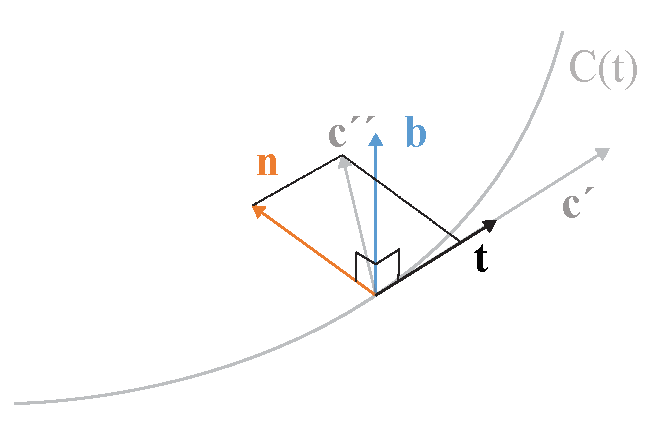
\includegraphics[width=0.7\linewidth ]{figure/Theory/CurveGeometry.pdf}              
\caption{The geometry of the curve, from Presley }
\end{figure}


\begin{equation}
\textbf{c}' =  \frac{d C(t)}{dt}, \quad \textbf{c}''=   \frac{d^2 C(t)}{dt^2}
\end{equation}


\begin{equation}
\textbf{t} = \frac{\textbf{c}'}{||\textbf{c}'||} 
\end{equation}

Since \textbf{c}´´ and \textbf{t} lies in the same plane one can get the vector \textbf{b} taking the cross product of \textbf{c}´´ and \textbf{t}. 
\begin{equation}
\textbf{b} = \frac{\textbf{t} \times \textbf{c}''}{||\textbf{t} \times \textbf{c}''||} 
\end{equation}

You have the following relations between the vectors.

\begin{equation}
\textbf{b} = \textbf{t} \times \textbf{n} ,\quad \textbf{n} = \textbf{b} \times \textbf{t} ,\quad \textbf{t} = \textbf{n} \times \textbf{b} 
\end{equation}

\subsubsection{Curvature and Torsion} \label{curvature}

\textit{Curvature} can be seen as a measure of how much a curve deviates from a straight line,Bär, or as Struik defines it as a measure of the rate of change of the tangent moving along the curve. \textit{Torsion} is a measure of the rate of change of the osculating plane, according to Struik.

\vspace{5mm} %5mm vertical space

Definition of curvature, $\kappa$, for regular curves can be described. 
\begin{equation}
\kappa = \frac{|| \textbf{c}'' \times \textbf{c}' ||}{||\textbf{c}'||^3} 
\end{equation}

Definition of torsion,$\tau$, for regular curves can be described. 
\begin{equation}
\tau = \frac{ \textbf{c}''' \cdot(\textbf{c}' \times \textbf{c}'')}{||\textbf{c}' \times \textbf{c}''||^2} 
\end{equation}

\subsection{Surfaces}

"The word "surface" is an important term in mathematics and is used in many ways. The most common and straightforward use of the word is to denote a two-dimensional submanifold of three-dimensional Euclidean space. Surfaces can range from the very complicated (e.g., fractals such as the Mandelbrot set) to the very simple (such as the plane). " Rewrite

\begin{figure}[H]
\centering
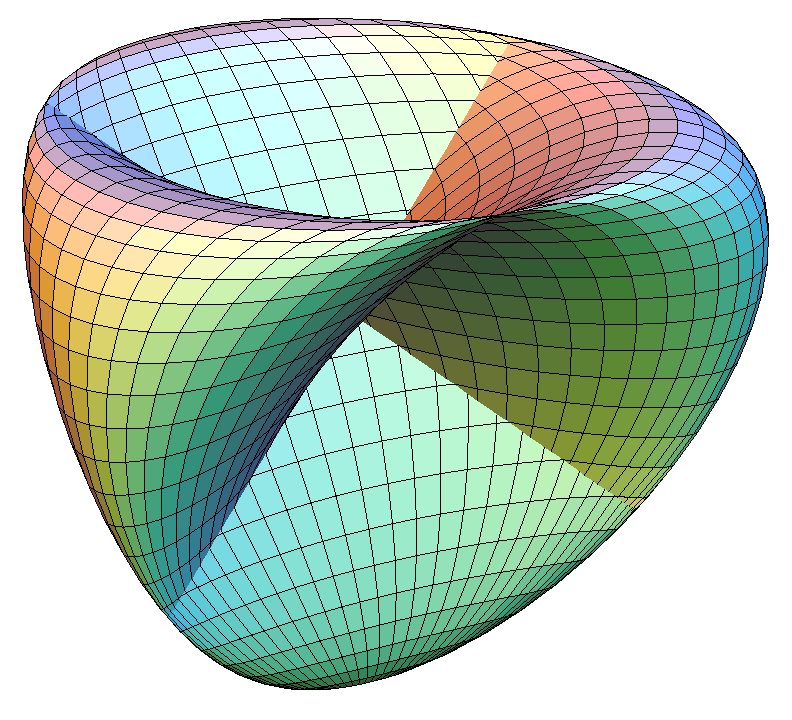
\includegraphics[width=0.5\linewidth]{figure/Theory/Romansurface.png}
 
\caption{Roman Surface $ x^2 y^2+x^2 z^2-x y z+y^2 z^2 = 0,$  }
\end{figure}





A mathematical definition for a regular surface can be written according to,Bär, as:

\vspace{5mm} %5mm vertical space

Let $S$  be a subset of $\mathbb{R}^3$ if there exists for every point $p \in S$ an open neighbourhood of $V$  of $p$ in $\mathbb{R}^3$, and if , in addition, there exists an open subset $U \subset \mathbb{R}^2$ and a smooth map $F:U \rightarrow \mathbb{R}^3$ such that
 
\begin{enumerate}
\item $ F(U) = S \cap V$  and $F:U \rightarrow S \cap V$ is a homeomorphism 
\item  the Jacobian $D_u F$ has rank 2 for every point $u \in U$  

\end{enumerate}


\begin{figure}[H]
\centering
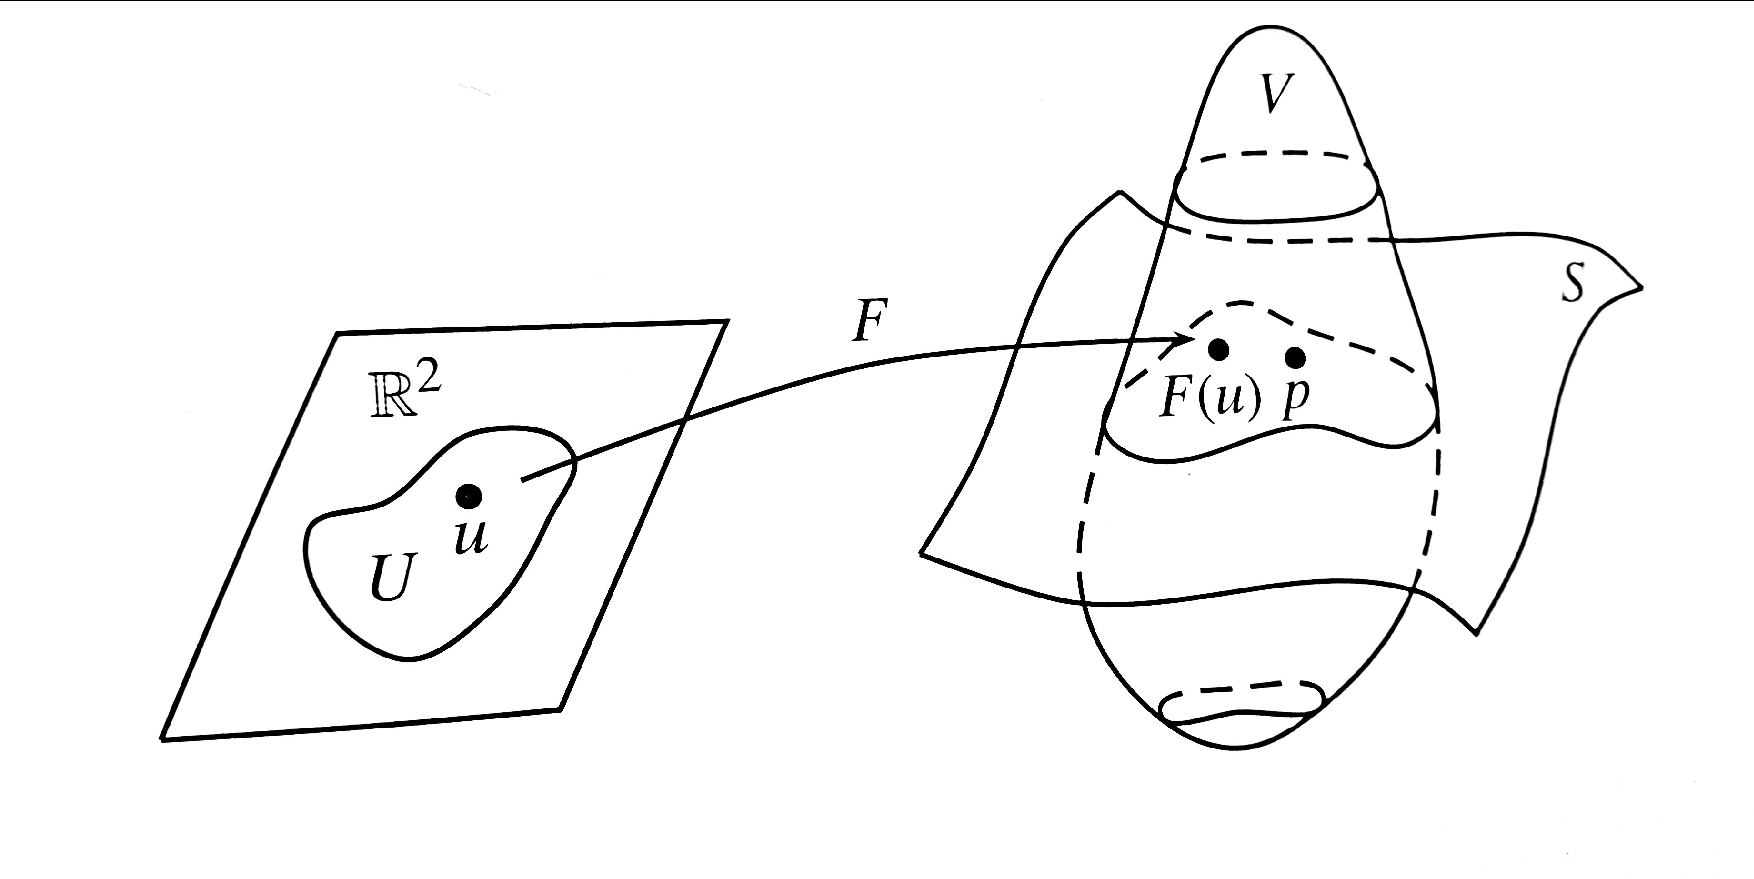
\includegraphics[width=0.7\linewidth]{figure/Theory/surfdef.pdf}
 
\caption{The tangent differs depending of which direction you refer to. }
\end{figure}


\begin{figure}[H]
\centering
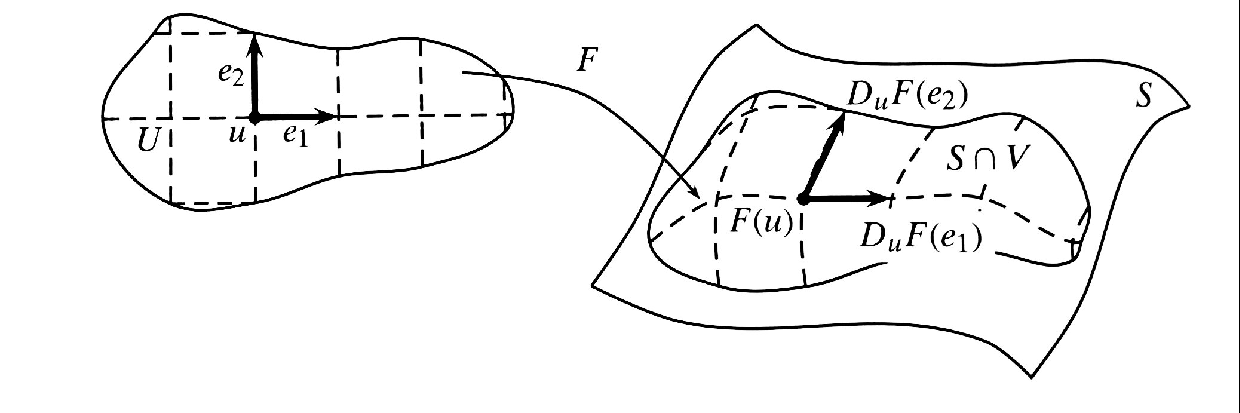
\includegraphics[width=0.8\linewidth]{figure/Theory/surffunction.pdf}
 
\caption{The tangent differs depending of which direction you refer to. }
\end{figure}




The most common surface is probably sphere which can be described in Cartesian coordinates as $ x^2 + y^2 + z^2 = R^2$ , where $R$ is the radius of the Sphere.

\begin{figure}[H]
\centering
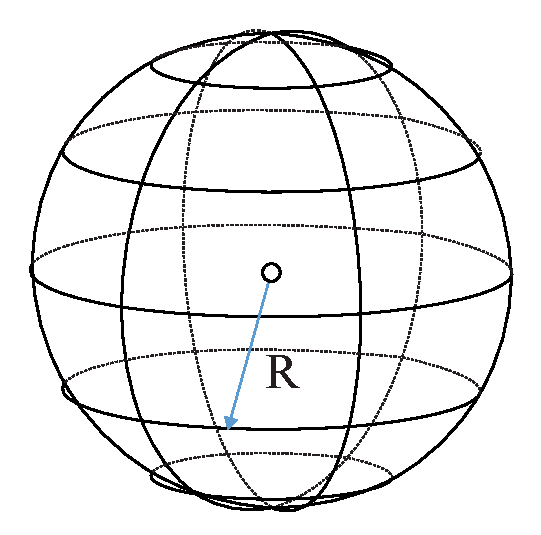
\includegraphics[width=0.4\linewidth ]{figure/Theory/sphereEx.pdf}                \caption{The tangent differs depending of which direction you refer to. }
\end{figure}

A general surface described in vector form as:
\begin{equation}
\textbf{r}(\theta^1,\theta^2) = x(\theta^1,\theta^2)\textbf{i} +  y(\theta^1,\theta^2)\textbf{j}+  z(\theta^1,\theta^2)\textbf{k}
\end{equation}

Where \textbf{i},\textbf{j} and \textbf{k} are base vectors and where $\theta^1$ and $\theta^2$ are the surface coordinates.



Writing the above example in this form would be:
\begin{equation}
x = R cos(\theta^1) sin (\theta^2),\quad
y = R  sin(\theta^1) cos (\theta^2),\quad
z = R sin(\theta^2)
\end{equation}

\subsubsection{Geometry on a Surface}

Describe the nets on the surface .....

To orientate and describe geometry on the surface we can use two pair of base vectors....

The covaraiant base vectors of the surface are:
\begin{equation} \label{convariantDiff}
 \textbf{a}_\alpha = \frac{\partial\textbf{r}}{\partial \theta^\alpha } = \frac{\partial x}{\partial \theta^\alpha }\textbf{i} + \frac{\partial y}{\partial \theta^\alpha }\textbf{j}+\frac{\partial z}{\partial \theta^\alpha }\textbf{k} = \textbf{r},_{\alpha} , for\quad \alpha = 1,2
\end{equation}


The covariant base vectors are rarily orthogonal to each other.

The contravaiant base vectors also lies in the plane of the surface and are defined by

\begin{align}
\textbf{a}_{\alpha} \cdot \textbf{a}^\beta = \delta^{\beta}_\alpha \\
\textbf{a}_{\alpha} \cdot \textbf{a}^3 = 0    
\end{align}

Where $\delta^{\beta}_\alpha$ is called a \textit{Kronecker delta} and has the properties $\delta^{\beta}_\alpha = 0$ if $\alpha \neq  \beta$ and $\delta^{\beta}_\alpha = 1$ if $\alpha =  \beta$. 
 
\begin{figure}[H]
\centering
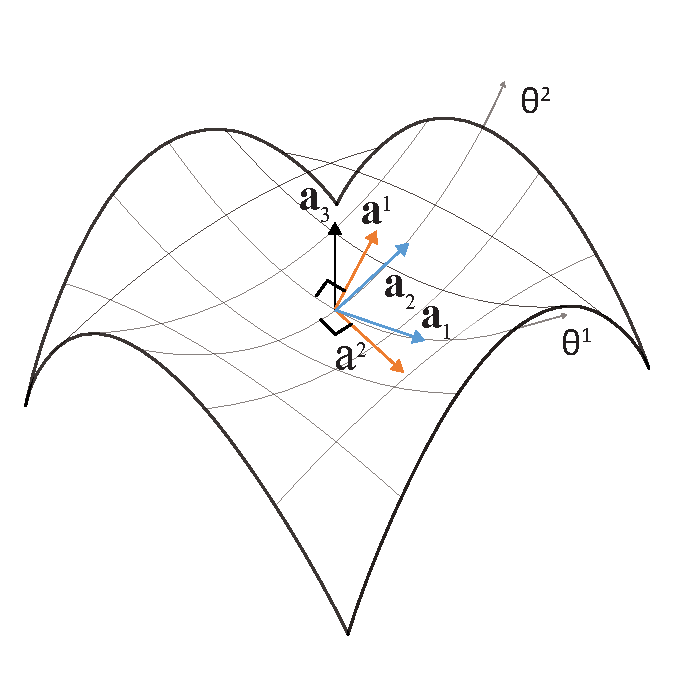
\includegraphics[width=0.7\linewidth ]{figure/Theory/surfGeometry2.pdf}
\caption{The tangent differs depending of which direction you refer to. }
\end{figure}
 
The components of the metric tensors can be defined as

\begin{align} \label{metricComp}
a_{\alpha \beta} = \textbf{a}_\alpha \cdot \textbf{a}_\beta \\
a^{\alpha \beta} = \textbf{a}^\alpha \cdot \textbf{a}^\beta 
\end{align}

The quantity $a$ can be seen as the determinant of the covaraiant metric tensor.

\begin{equation}
a = a_{11} a_{22} + a_{12}^2
\end{equation}



The use of the two sets of base vectors can be shown be illustrated by this example, Willams. By specifying an vector $\textbf{p}$ it can be written in both contravariant and covariant base vectors.

\begin{equation}
    \textbf{p} = p_x \textbf{i} +p_y \textbf{j} +p_z \textbf{k}  
\end{equation}
\begin{equation}
    \textbf{p} = p^\alpha \textbf{a}_\alpha + p \textbf{a}^3 =   p^1 \textbf{a}_1 +  p^2 \textbf{a}_2 + p \textbf{a}^3 
\end{equation}
\begin{equation}
    \textbf{p} = p_\alpha \textbf{a}^\alpha + p \textbf{a}^3=  p_1 \textbf{a}^1 +  p_2 \textbf{a}^2 + p \textbf{a}^3   
\end{equation}


\begin{figure}[H]
\centering
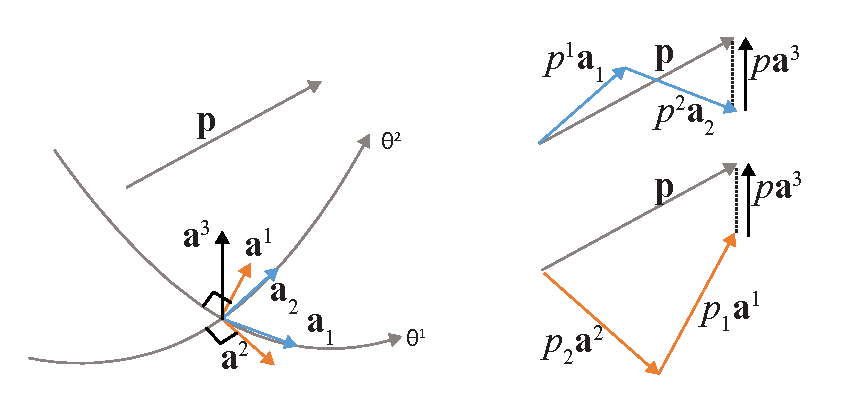
\includegraphics[width=0.8\linewidth ]{figure/Theory/Covariant.pdf}
\caption{The tangent differs depending of which direction you refer to. }
\end{figure}




\subsubsection{First fundamental Form}

The First Fundamental is the measure of the length of a surface. This is an intrinsic property since the length always is the same for real surfaces. It can tell us how the measures will be behave on the surface. For example a plane and a cylinder has the same first fundamental form which means that  a line drawn on a paper has the same length as the curve on the folded cylinder by the same paper.

\begin{figure}[H]
\centering
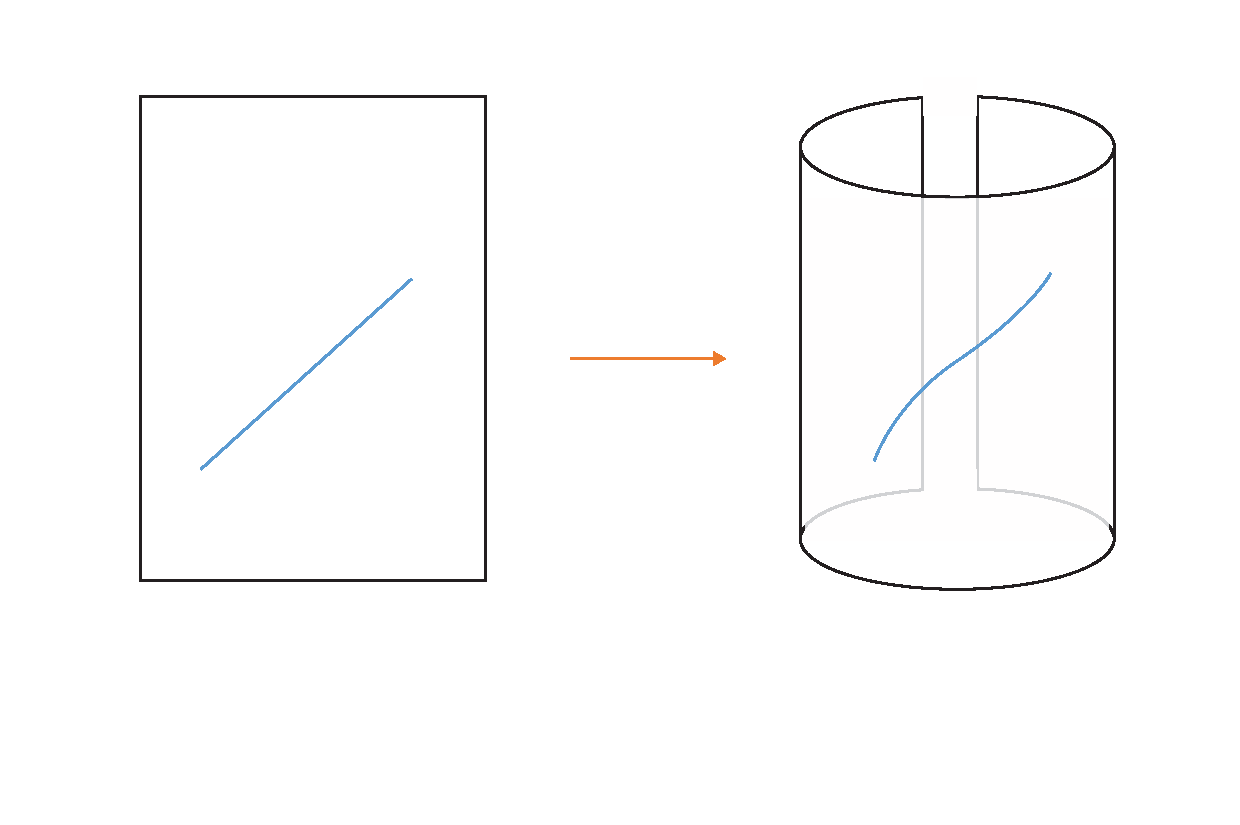
\includegraphics[width=0.9\linewidth ]{figure/Theory/FirstFundamental.pdf}
\caption{The tangent differs depending of which direction you refer to. }
\end{figure}

The plane and the sphere for example does not have the same first fundamental form which is why we can not form a paper directly to a sphere without modifications. Therefore a curve drawn on the sphere would not have a true relation to the plane as the cylinder and the plane has.

\begin{figure}[H]
\centering
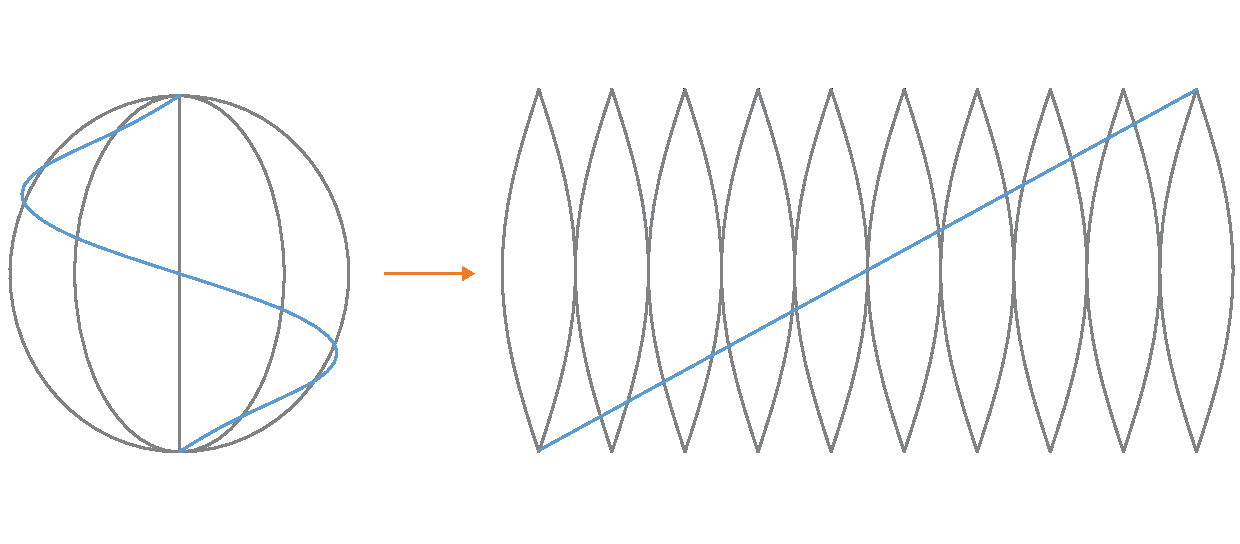
\includegraphics[width=0.9\linewidth ]{figure/Theory/unrollSurfMod.pdf}
\caption{The tangent differs depending of which direction you refer to. }
\end{figure}


If we were to measure the line length from P and Q which is say $\delta s$. Then 

\begin{equation}
\delta s^2 = \delta \textbf{r} \cdot \delta \textbf{r} =  \textbf{a}_\alpha \cdot \textbf{a}_\beta \delta\theta^\alpha \delta\theta^\beta =  \textbf{a}_{\alpha\beta} \delta\theta^\alpha \delta\theta^\beta 
\end{equation}

The components of the covariant metric tensor $a_{\alpha \beta}$ described in \ref{metricComp} are also what is called the coefficients of the \textit{first fundamental form}.
It is common that these are described differently in math literature such as Struik which uses the following notation:
$$ E= a_{11} ,\quad  F = a_{12},\quad
 G = a_{22}$$

The curve distance P and Q can be described as following for a curve $ \textit{C}(t) = \textbf{r}(\theta^1(t),\theta^2(t))$:

$$s = \int { \sqrt { a_{11} \Big(\frac{d\theta^1 }{dt}\Big)^2+2a_{12}\Big(\frac{d\theta^1 }{dt}\Big)\Big(\frac{d\theta^2 }{dt}\Big)  +a_{22} \Big(\frac{d\theta^2 }{dt}\Big)^2 }  } dt$$



\subsubsection{Second fundamental Form}

The second fundamental form is the measure of the deviation from a tangent plane, Stokes.

\begin{figure}[H]
\centering
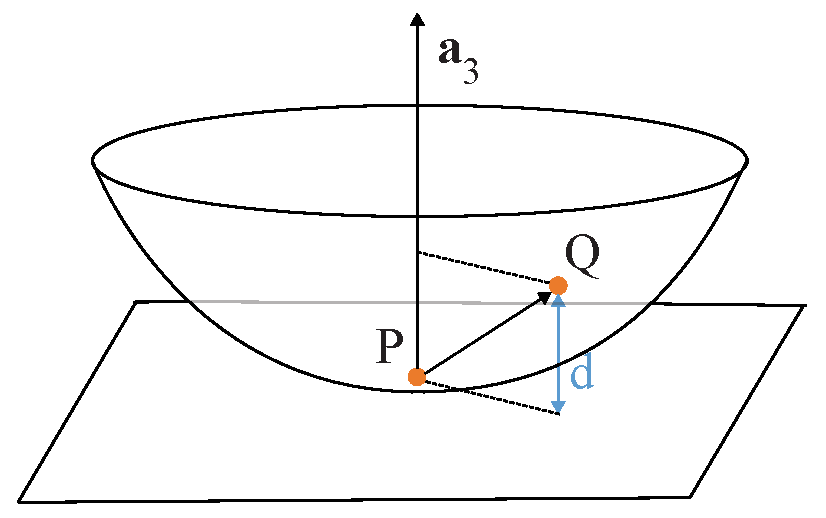
\includegraphics[width = 0.7\linewidth ]{figure/Theory/SecondFFil.pdf}
\caption{http://web.mit.edu/hyperbook/Patrikalakis-Maekawa-Cho/node29.html}
\end{figure}

Suppose we have points P and Q on the surface that are described as $r(\theta^1, \theta^2)$ and $r(\theta^1 + d\theta^1, \theta^2 + d\theta^2)$.

A taylor expansion of $r(\theta^1 + d\theta^1, \theta^2 + d\theta^2)$.

$$
\textbf{r}(\theta^1 + d\theta^1, \theta^2 + d\theta^2)= \textbf{r}(\theta^1, \theta^2) + \textbf{r}_{,1} d\theta^1 + \textbf{r}_{,2} d\theta^2 + \frac{1}{2}(\textbf{r}_{,11}(d\theta^1)^2 + 2\textbf{r}_{,12}d\theta^1 d\theta^2 + \textbf{r}_{,11}(d\theta^2)^2) + remainder
$$

Therefore \textbf{PQ} can be described as
$$
\textbf{PQ} = r(\theta^1 + d\theta^1, \theta^2 + d\theta^2) - r(\theta^1, \theta^2) =  \textbf{r}_{,1} d\theta^1 + \textbf{r}_{,2} d\theta^2 + \frac{1}{2}(\textbf{r}_{,11}(d\theta^1)^2 + 2\textbf{r}_{,12}d\theta^1 d\theta^2 + \textbf{r}_{,11}(d\theta^2)^2) 
$$

Projecting PQ onto $\textbf{a}^3$ 
$$
d = \textbf{PQ}\cdot\textbf{a}^3 = \frac{1}{2}(\textbf{r}_{,11}(d\theta^1)^2 + 2\textbf{r}_{,12}d\theta^1 d\theta^2 + \textbf{r}_{,11}(d\theta^2)^2) \cdot \textbf{a}^3 
$$

This is due to $(\textbf{r}_{,1} d\theta^1 + \textbf{r}_{,2}d\theta^2)\cdot\textbf{a}^3 = 0$

Recall from equation \ref{convariantDiff} that $\textbf{r}_\alpha = \textbf{a}_\alpha$ And that $a_{\alpha\beta}$ are the coefficents of the first fundamental form. In similar fashion we define the coefficents of the Second fundamental form $b_{\alpha\beta}$ 

\begin{equation}
b_{\alpha\beta} = \textbf{a}_3 \cdot \textbf{a}_{\alpha,\beta} 
\end{equation}

Applying this the second fundamental form can be written as:

$$ ~\upperRomannumeral{2} = b_{11}(d\theta^1)^2 + 2b_{12}d\theta^1 d\theta^2 + b_{22}(d\theta^2)^2 = -d\textbf{r}\cdot d\textbf{a}_3$$

Reading literature by Presley, Stokes and Struik they have another definition, but it can be related like this.
$$ e = L = b_{11} ,\quad  f= M = b_{12},\quad
 g = M = b_{22}$$


It is appropriate to distinguish four different cases depending on the determinant

\begin{itemize}
\item $b_{12}^2 - b_{11}b_{22} > 0$ \\
Text text text.....
\item $b_{12}^2 - b_{11}b_{22} = 0$ \\
Text text text.....
\item $b_{12}^2 - b_{11}b_{22} < 0$ \\
Text text text.....
\item $b_{12} = b_{11} = b_{22} = 0$ \\
Text text text.....
\end{itemize}



\begin{figure}[H]
\centering
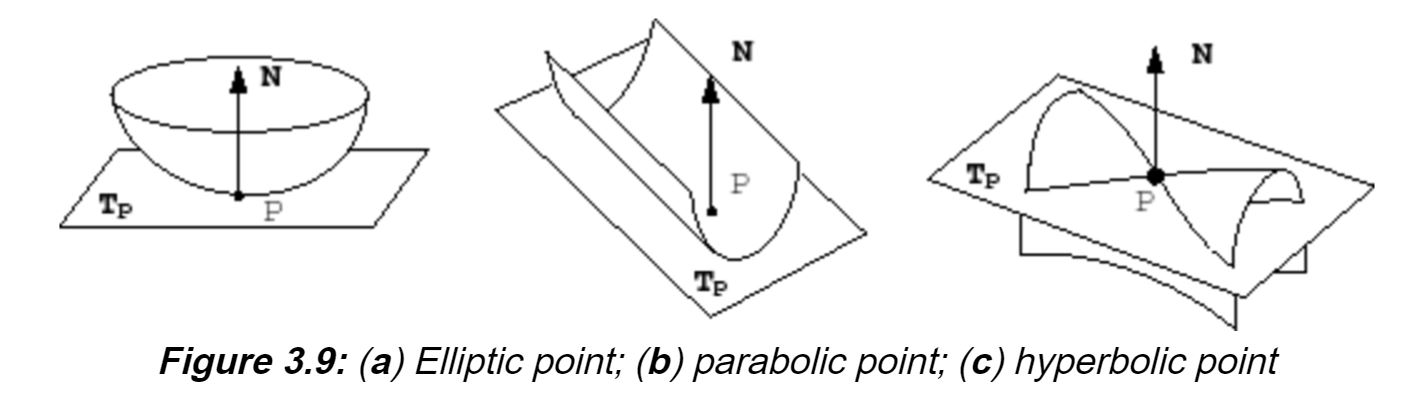
\includegraphics[width = 1\linewidth ]{figure/Theory/SecondFF2.JPG}
\caption{http://web.mit.edu/hyperbook/Patrikalakis-Maekawa-Cho/node29.html}
\end{figure}

\subsubsection{Christoffel Symbols}

Christoffel Symbols are defined and used to measure the rate of change from a point P to a point Q in the base vectors of P.



In the book  \textit{Einstein's Theory: A Rigorous Introduction for the Mathematically Untrained}, you can read this description \textit{ "The Christoffel symbol $\Gamma^\gamma_{\alpha \beta}$, is the $\gamma$ component of the change of the coordinatebasis vector $ \textbf{a}_\beta $ by an infinitesimal coordinate displacement $ d\theta^\alpha $, per unit coordinate
distance."} 

With this definition:

\begin{equation}
\Gamma^\gamma_{\alpha \beta} = \frac{\partial\textbf{a}_\beta}{\partial\theta^\alpha}\cdot \textbf{a}^\gamma
\end{equation}



"They give the properties of the coordinate system as lengths and directions change along the coordinate curves. They do not represent anything real, are NOT the components of a tensor and do not obey the tensor component rule under a change of coordinates." Chris Willams

\begin{figure}[H]
\centering
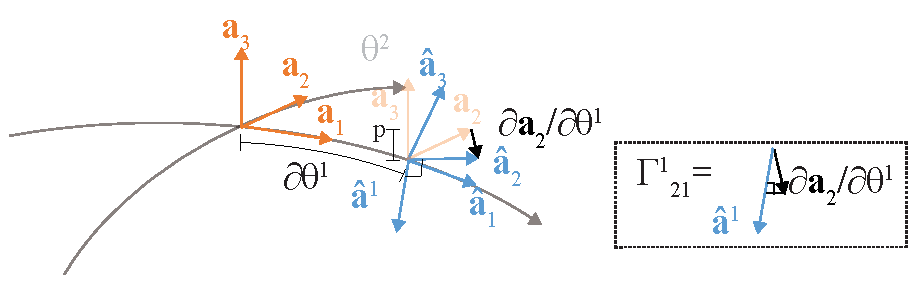
\includegraphics[width=0.9\linewidth ]{figure/Theory/christoffelSecondKind.pdf}
\caption{ Geometric representation of Christoffel Symbol of Second kind }
\end{figure}

\begin{figure}[H]
\centering
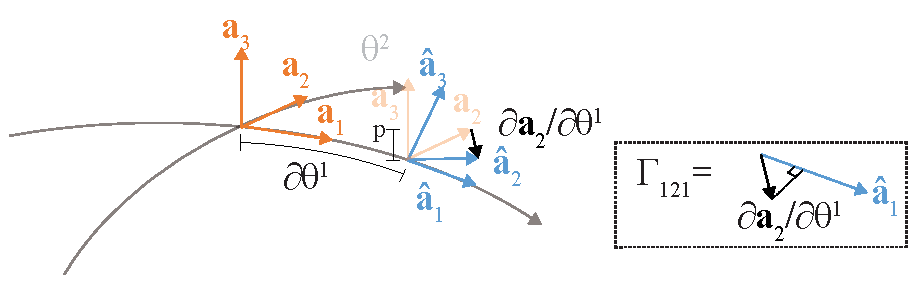
\includegraphics[width=0.9\linewidth ]{figure/Theory/christoffelFirstKind.pdf}
\caption{Geometric representation of Christoffel Symbol of First kind }
\end{figure}

In 3d:

\begin{equation}
 \frac{\partial\textbf{g}_i}{\partial\theta^j} = \Gamma^k_{i j} \textbf{g}_k 
\end{equation}

For a surface:

\begin{equation}
    \frac{\partial\textbf{a}_\beta}{\partial\theta^\alpha} = \Gamma^\lambda_{\alpha \beta} \textbf{a}_\lambda + b_{\alpha \beta}\textbf{a}_3
\end{equation}



\subsubsection{Gauss-Codazzi Equations}

Chris Williams states in Use of structural analogy
generation of smooth
surfaces for engineering
purposes. \textit{ "The Gauss-Codazzi equations (Gauss' theorem and the
Codazzi equations) are compatibility equations, which
ensure that the coefficients of the first and second fundamental
forms are related in such a way that the surface
'fits together'."} 




In Green and Zerna you can read the following defintion of the Codazzi
equations:
\begin{equation}
    b_{\alpha 1}|_2 = b_{\alpha 2}|_1 
\end{equation}

In Struik we can read them as:

\begin{equation}
   b_{11},_2 - b_{12},_1 = b_{11} \Gamma^1_{12} + b_{12}(\Gamma^2_{12} - \Gamma^1_{11}) - b_{22}\Gamma^2_{11} 
\end{equation}

\begin{equation}
   b_{12},_2 - b_{22},_1 = b_{11} \Gamma^1_{22} + b_{12}(\Gamma^2_{22} - \Gamma^1_{12}) - b_{22}\Gamma^2_{12} 
\end{equation}


\begin{equation}\label{Gauss}
  K= \frac{b_{11}b_{22}-b^2_{12}}{a}
\end{equation}

\begin{equation}
  K= \frac{1}{4}\epsilon^{\lambda \alpha} \epsilon^{\beta \gamma} \bar{R}_{\lambda \alpha \beta \gamma}
\end{equation}

Where Green and Zerna calls $\bar{R}_{\lambda \alpha \beta \gamma}$ the  \textit{associated Riemann-Christoffel tensor} which is defined as.

\begin{equation}
 \bar{R}_{\lambda \alpha \beta \gamma} = a_{\lambda \mu} \bar{R}^\mu_{.\alpha \beta \gamma}
\end{equation}

 Where $\bar{R}^\mu_{.\alpha \beta \gamma}$ which is called the \textit{Riemann-Christoffel tensor} can be written in Christoffel Symbols.
\begin{equation} \label{Gauss2}
\bar{R}^\lambda_{.\alpha \beta \gamma} = \Gamma^3_{\alpha \beta} \Gamma^\lambda_{3\gamma}-\Gamma^3_{\alpha \gamma}\Gamma^\lambda_{3\beta} 
\end{equation}

Equation \ref{Gauss2} shows what \ref{Gauss} can be written in terms of the first fundamental form, since Christoffel symbols can be written in the first fundamental form components.


\subsubsection{Principal Curvature}

The directions in the tangent plane for which $\kappa_n$ takes maximum takes maximum and minumum values are called principal directions. Struik


\begin{figure}[H]
\centering
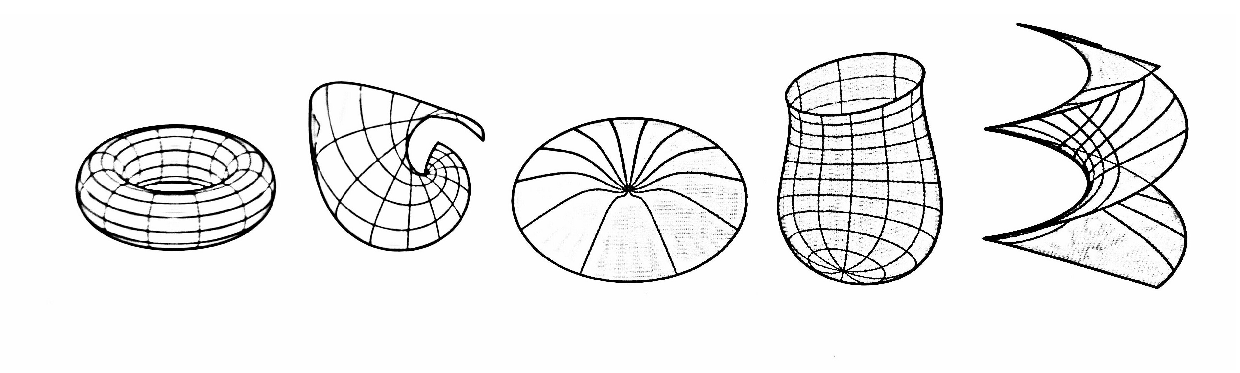
\includegraphics[width = 0.9\linewidth ]{figure/Theory/principalCurvature.pdf}
\caption{Scan better picture from Pottman }
\end{figure}


\subsubsection{Gaussian and Mean Curvature}

Two measures to describe the curveature of a surface are what is called Gaussian and Mean Curvature. It can be described in the forms of the principal curvature. Both can though be written in terms of first and second fundamental form as well.

The mean curvature, $H$, is the mean curvature of the principal curvature
\begin{equation}
H = \frac{\kappa_1 + \kappa_2}{2} =\frac{b_{11}b_{22} - 2b_{12}a_{12} + b_{22}a_{11}}{2(a_{11}a_{22} - (a_{12})^2)}
\end{equation}

The Gaussian curvature, K, is the product of the two
principal curvatures.

\begin{equation}
K = {\kappa_1 \kappa_2} = \frac{b_{11} b_{22} - (b_{12})^2}{a_{11}a_{22} - (a_{12})^2}
\end{equation}

The geometrical meaning of the Gaussian curvature can be seen in below.  A point of positive Gaussian curvature is a point where you have positive principal curvature in both directions as in a sphere. This is a point where you have two parabolas who's openings are directed the same way. A negative Gaussian curvature means that you have two parabolas but where they are directed in opposite directions. Zero Gaussian curvature is a result of one or both Principal curvatures are zero as in a cylinder.

\begin{figure}[H] 
\centering
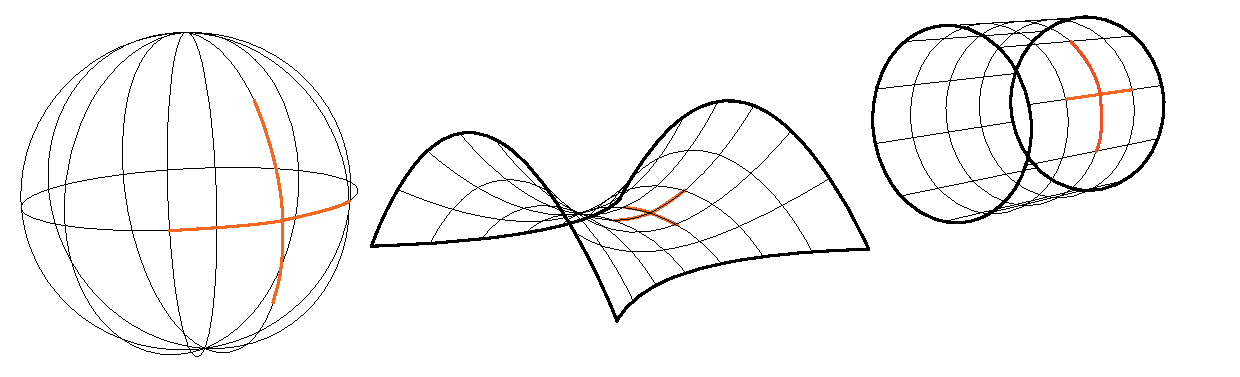
\includegraphics[width=1\linewidth ]{figure/Theory/GaussForms.pdf}
\caption{pottman}
\end{figure}

Surfaces of no Mean curvature is what we are calling minimal surfaces. Usually we define that as a surface of the smallest area spanned by a given closed space curve, even though this is not always true according to Struik. 
A minimal surface can be produced physically by using soap film and was experimented by Frei Otto. These experiments have quite similar properties as his works in architecture. 

\begin{figure}[H] 
\centering
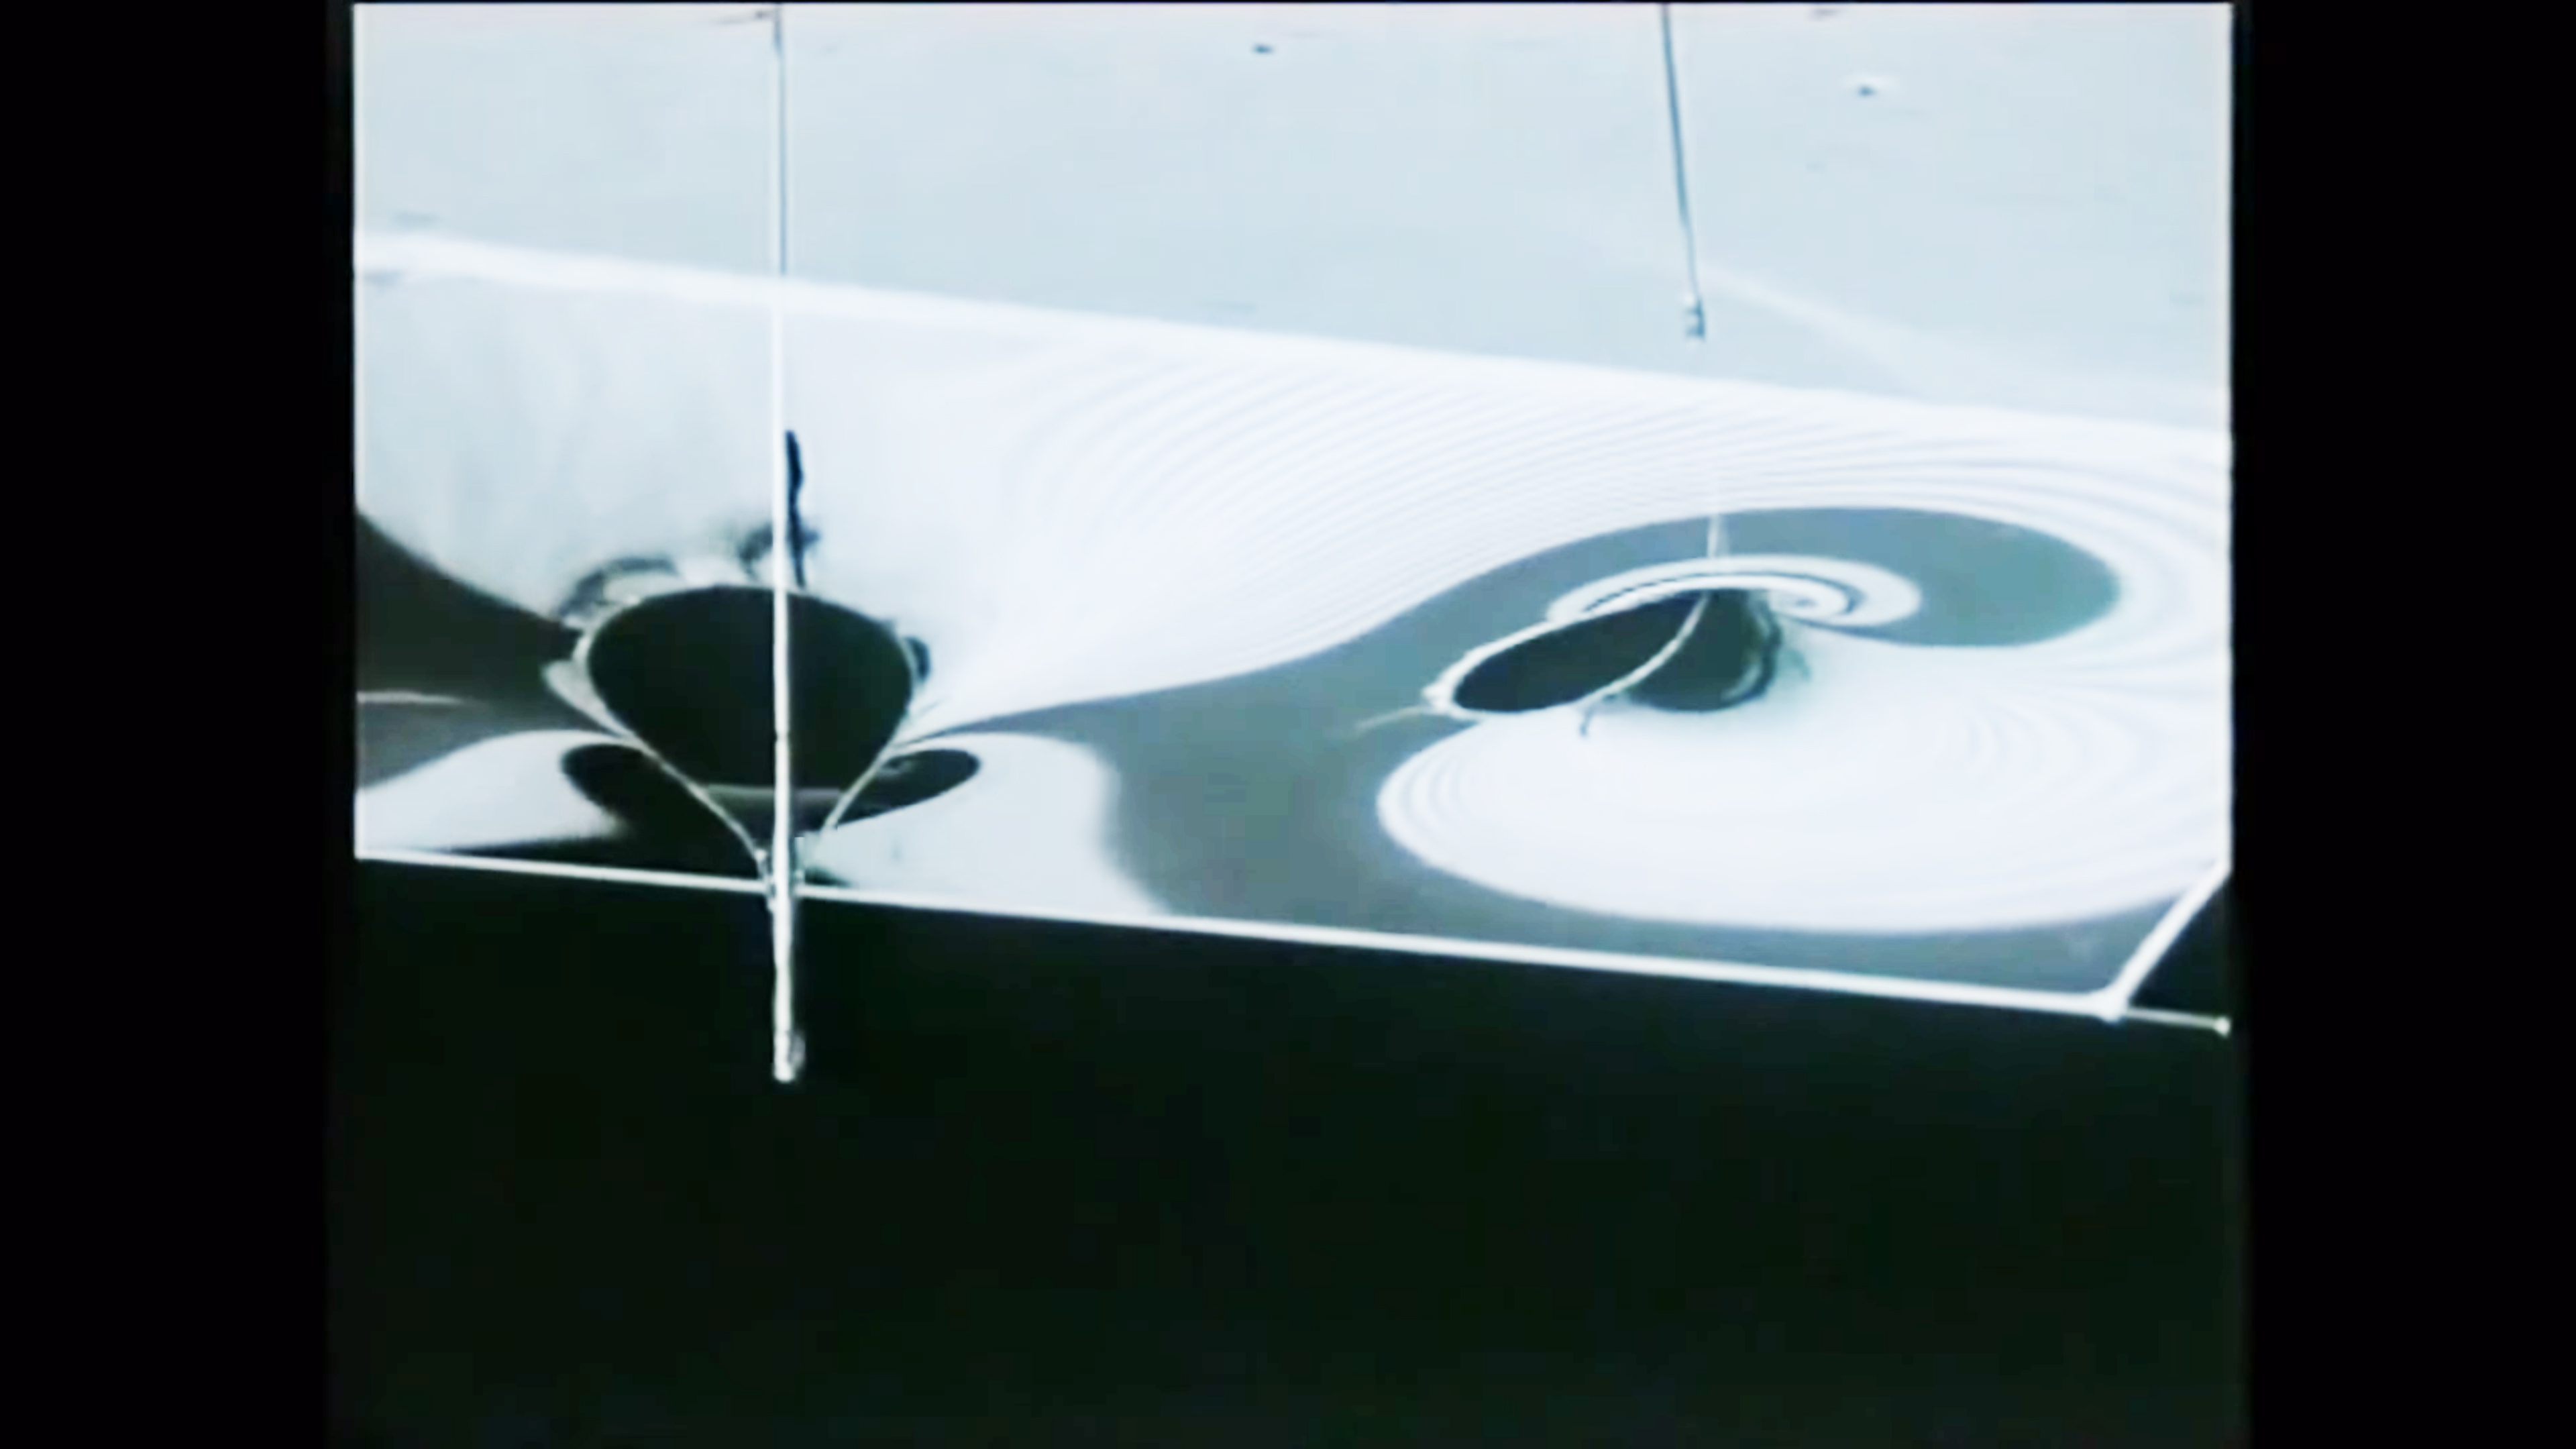
\includegraphics[width=0.9\linewidth ]{figure/Theory/SoapSreeen.jpg}
\caption{Screenshoot from a movie of Frei Ottos}
\end{figure}


\begin{figure}[H] 
\centering
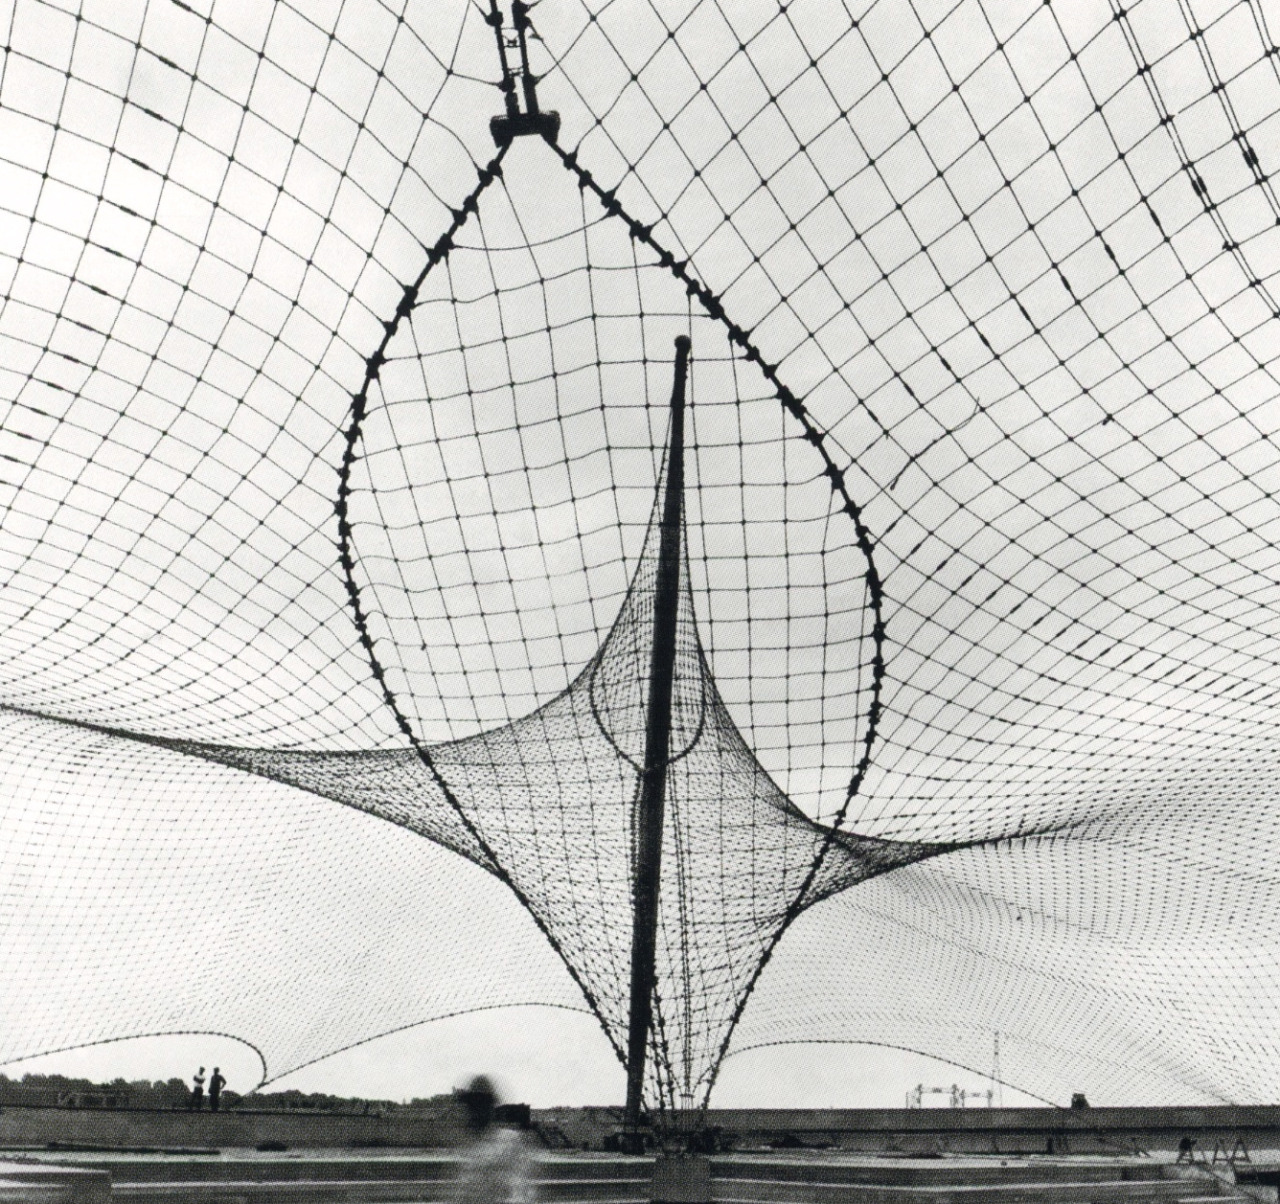
\includegraphics[width=0.9\linewidth ]{figure/Theory/FreiOtto.jpg}
\caption{Screenshoot from a movie of Frei Ottos}
\end{figure}



\subsection{Curves on Surfaces}

So far we have covered the properties of surfaces and curves somewhat separately. The properties of curves on surfaces differs, or how we describe them, a bit from the curves in  space. It is possible to relate the properties of the curve to the surface geometry, for instance you have a normal in every point of the curve. The most famous curve on the surface might for instance be the geodesic.

\begin{figure}[H]
\centering
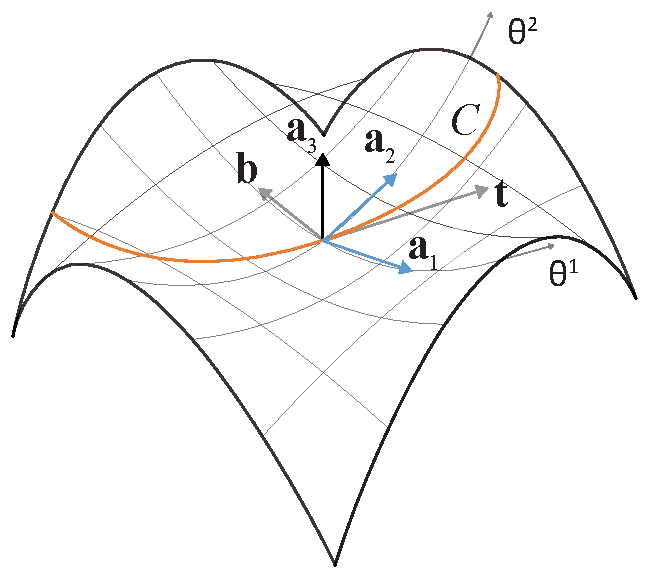
\includegraphics[width=0.7\linewidth ]{figure/Theory/CurveOnSurface.pdf}
\caption{The tangent differs depending of which direction you refer to. }
\end{figure}



\subsubsection{Geodesics}

A geodesic can be described as the the shortest path between two points, or "straight". Straight in this sense meaning the direction the car would go without turning the wheels. Though it might be hard to imagine a straight curve on a non flat surface. One way is to think of an ant moving on surface in what it perceives as an straight motion. (Skate park Example?) The most common geodesics are the great circles of a sphere. Presley 215

\begin{figure}[H]
\centering
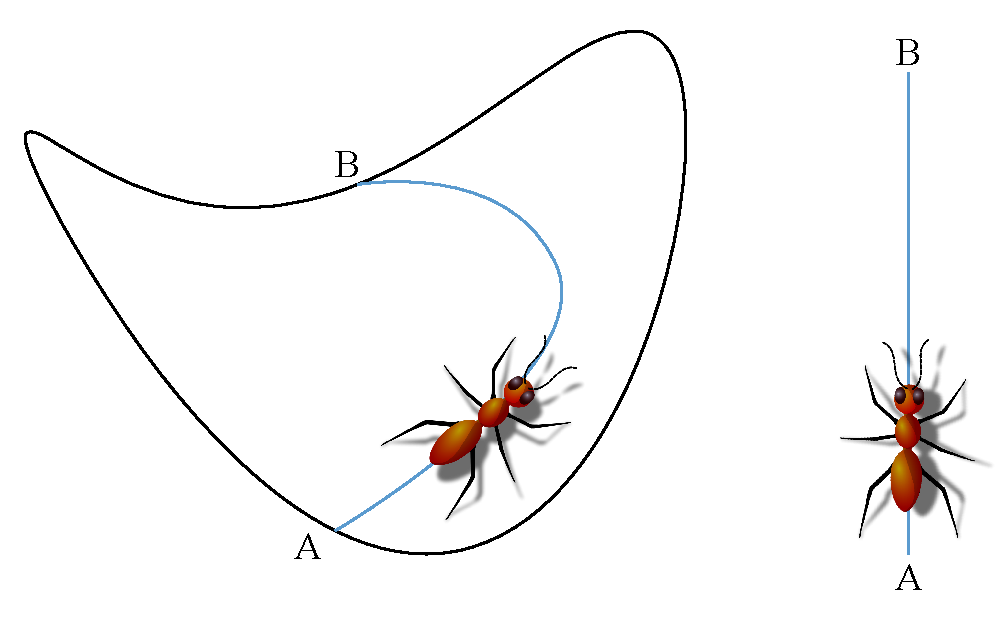
\includegraphics[width=0.7\linewidth ]{figure/Theory/Geodesics.pdf}
\caption{An ant moving on the surface in what it senses as a straight line is called a geodesic }
\end{figure}

So you can think of a geodesic as a shortest path between A and B but you can also say that standing in A there is a geodesic in every direction.\\
"\textit{Through every point of the surface passes a geodesic in every direction. A geodesic is uniquely determined by an initial point and tangent at that point}" Struik 133
To describe this in a mathematical way you would say that the geodesic curvature is zero in every point on the curve. 
Applications in Architecture is for instance to get the cutting patterns for tensile structure. You could also see the umbrella for this.


\begin{figure}[H]
\centering
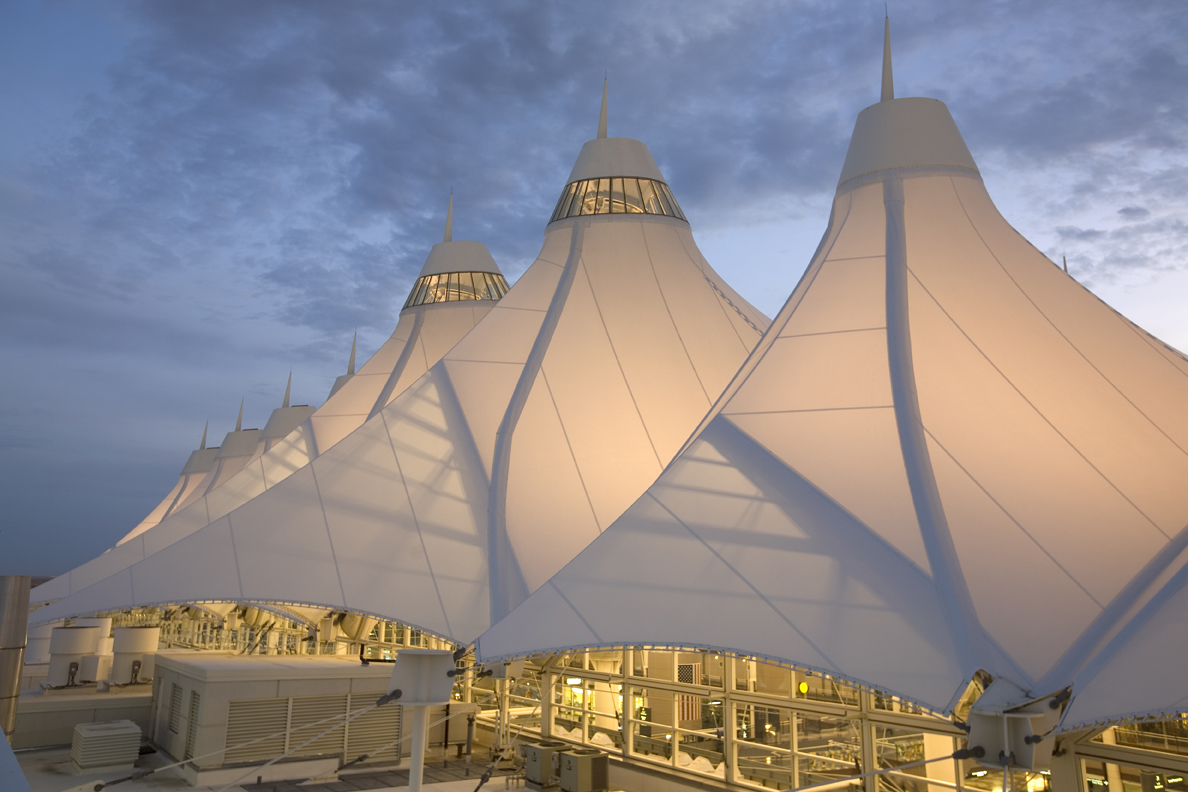
\includegraphics[width=0.9\linewidth ]{figure/Theory/Denver.jpg}

\caption{Airport of Denver with a membrane structure. You can see the cutting patterns of the structure. }
\end{figure}

\subsubsection{Normal and Geodesic Curvatures}

\begin{figure}[H]
\centering
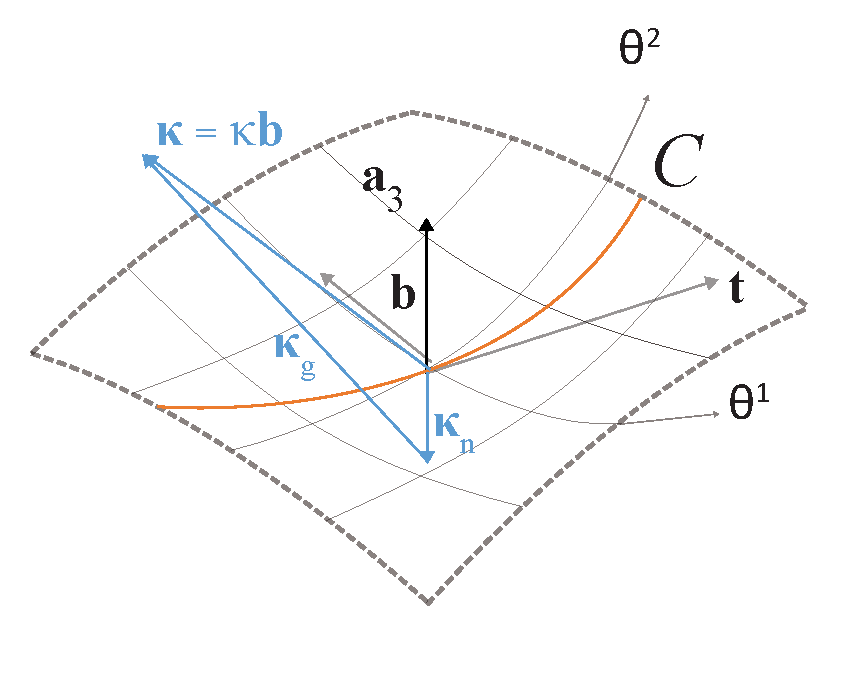
\includegraphics[height=0.6\linewidth ]{figure/Theory/SFF.pdf}
\caption{The tangent differs depending of which direction you refer to. }
\end{figure}

\subsection{Curve Linear Coordinates On The Surface}

Curve linear coordinates are... The properties of the different coordinate systems can be quite useful for practical reasons examples of those are ... .  

\subsubsection{Geodesic Coordinates}

Geodesic coordinates were introduced and extensively used by Gauss in his \textit{Disquisitones} of 1827.(Struik)The foundation of the geodesic coordinates is the  \textit{geodesic form}.\\ 
In Struik we can read \textit{"Equation \ref{geodesicForm} is called the 'geodesic form' of the line element and ($\theta^1,\theta^2$) form a set of 'geodesic coordinates'; or, for short, 'geodesic set'.On every surface we can find an infinte number of geodesic szets, depending on an arbeitrary curve $C_0$, along which the curves $\theta^2$ = constant can still be spaced in an arbitrary way."}\\

\begin{figure}[H]
\centering
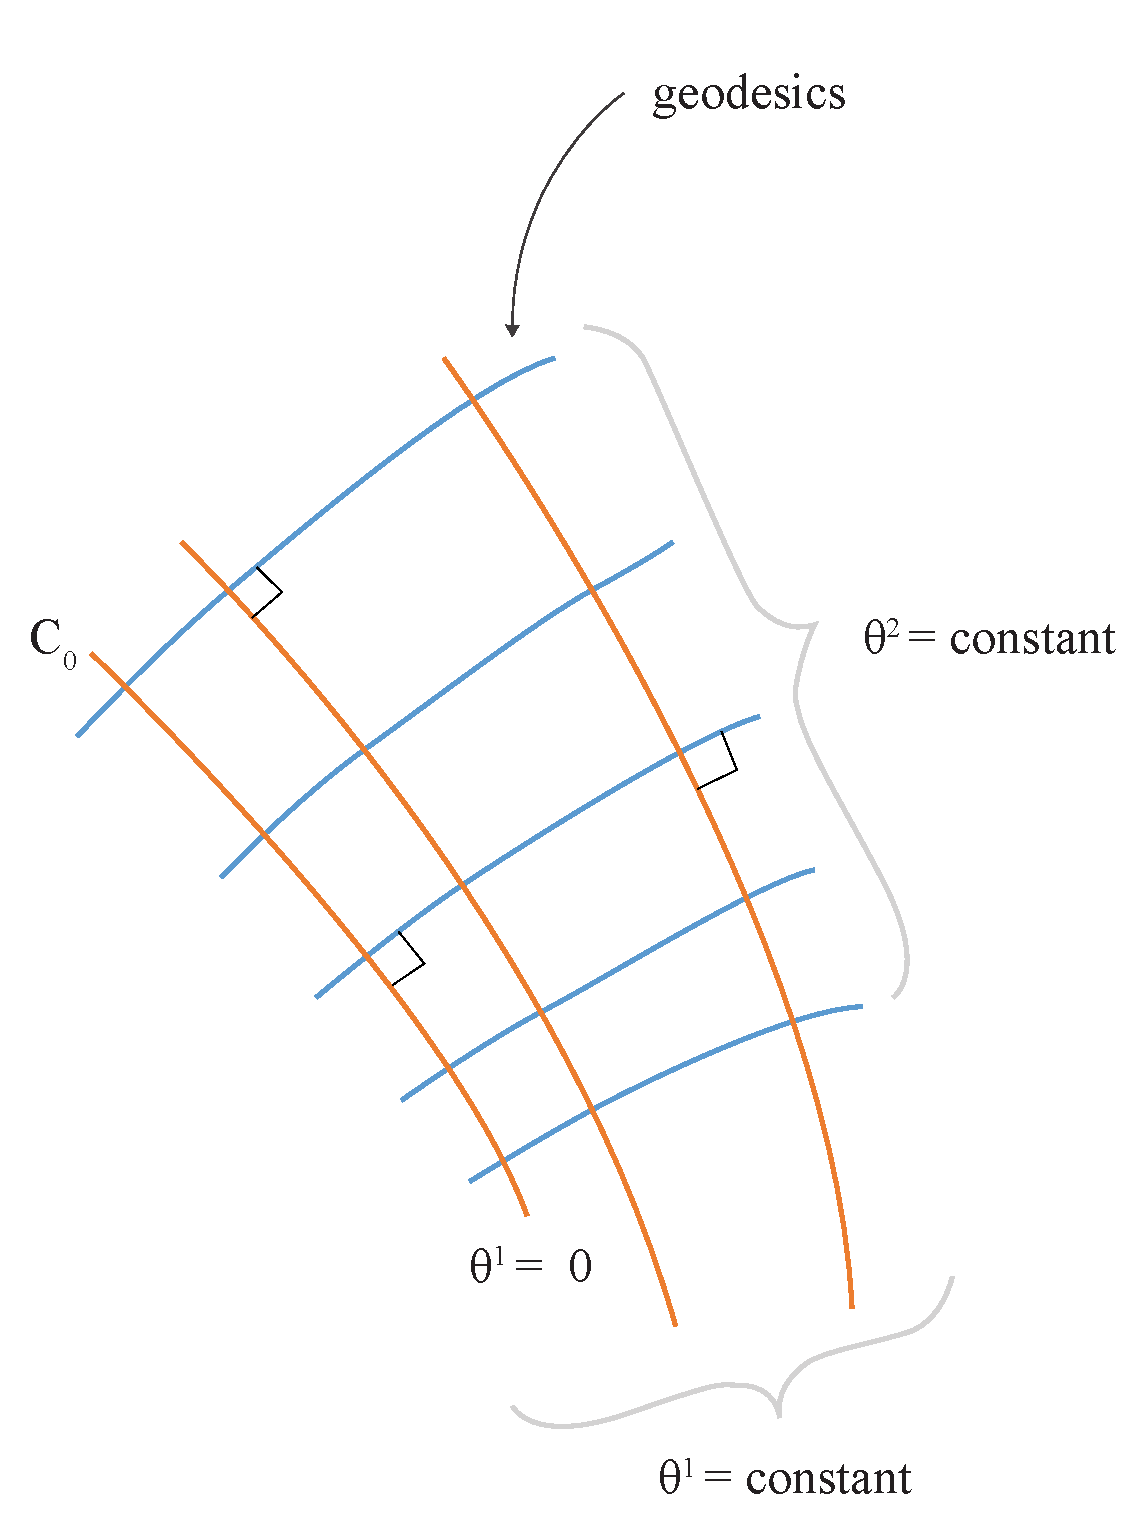
\includegraphics[height=0.8\linewidth ]{figure/Theory/geodesicCoordRe.pdf}
\caption{Redrawn picture from Struik }
\end{figure}


\begin{equation}\label{geodesicForm}
    ds^2 = (d\theta^1)^2 + a_{22}(\theta^1,\theta^2)(d\theta^2)^2
\end{equation}

In the geodesic form it states that $a_{11} = 1$ and $a_{12}=a_{21} = 0$. This means that $\textbf{a}_1$ and $\textbf{a}_2$ are perpendicular everywhere on the surface. 

Struik also states that the segments  on all geodesics included  between any to two orthogonal  trajectories are orthogonal.


\begin{figure}[H]
\centering
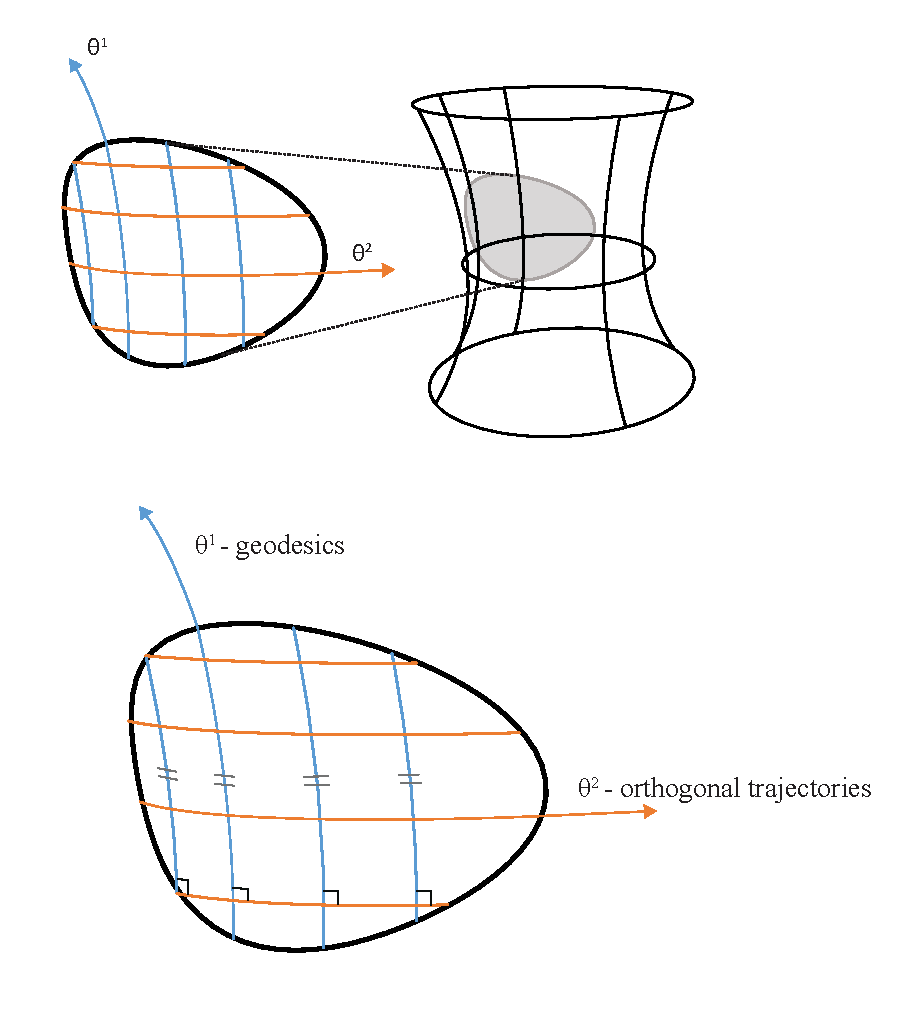
\includegraphics[height=0.8\linewidth ]{figure/Theory/SurfGeodesics.pdf}
\caption{The tangent differs depending of which direction you refer to. }
\end{figure}

This is possible to prove using Chris Williams approach to assume that you have a curve linear coordinate system where $a_{12} = 0$ and that $a_{22} = h^2 = constant$. That means that derivative must be equal to zero.

\begin{equation}
a_{12,2} = \textbf{a}_{1,2} \cdot \textbf{a}_2 + \textbf{a}_1 \cdot \textbf{a}_{2,2} = 0
\end{equation}
\begin{equation}
a_{22,1} = 2\textbf{a}_{2} \cdot \textbf{a}_{2,1} = 2\textbf{a}_{2} \cdot \textbf{a}_{1,2} = 0
\end{equation}

so that

\begin{equation}
\textbf{a}_1 \cdot \textbf{a}_{2,2} = 0
\end{equation}

Which means that the coordinate curves $\theta^1 = constant$ are geodesics. 


\subsubsection{Polar Geodesic Coordinates}

\begin{figure}[H]
\centering
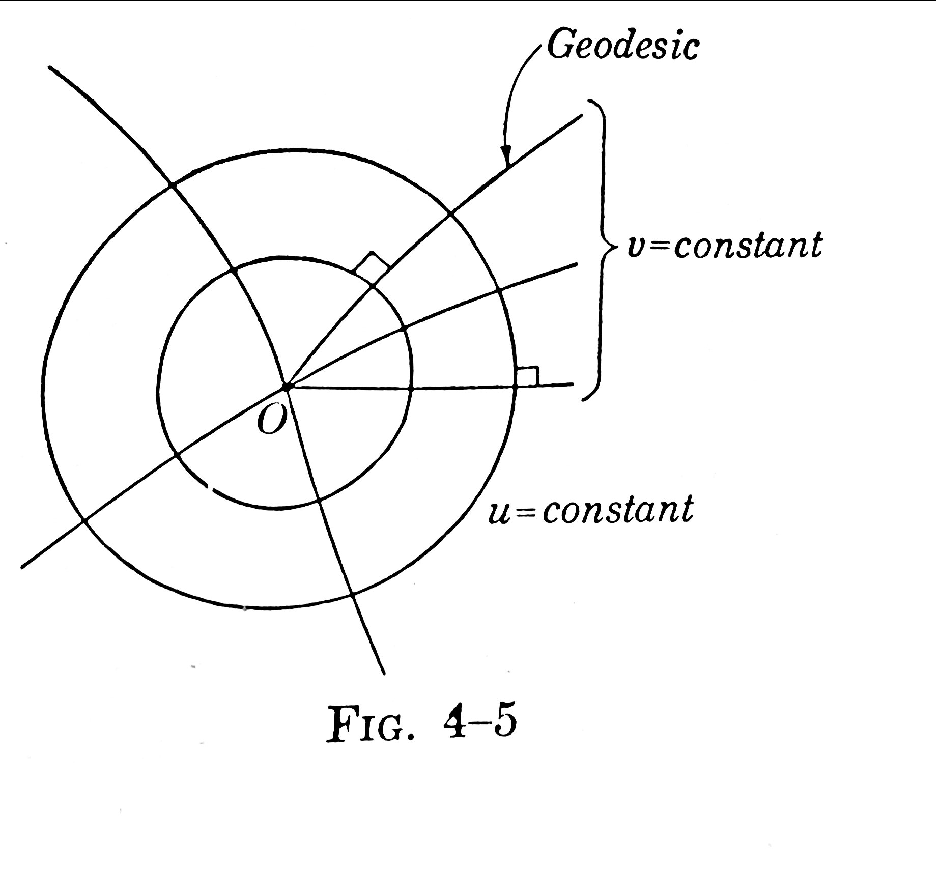
\includegraphics[height=0.5\linewidth ]{figure/Theory/polarGeodesicCoordMod.pdf}
\caption{The tangent differs depending of which direction you refer to. }
\end{figure}


\subsubsection{Equal Mesh Net Coordinates}

For a defined surface it is possible to apply an equal mesh net. They do not necessarily consist of squares but most likely of mostly rhombus. The constraint for this is that the angle is allowed to change to consist the equal lengths. This is describe in detail by Willams in his papper from 1980 and in the book shell Struc...\\
If the $a_{11} = a_{22} = L^2 = constant$ and $a_{12} = L^2\quad cos\alpha$ where $\alpha$ is the angle between the members.\\

\begin{figure}[H]
\centering
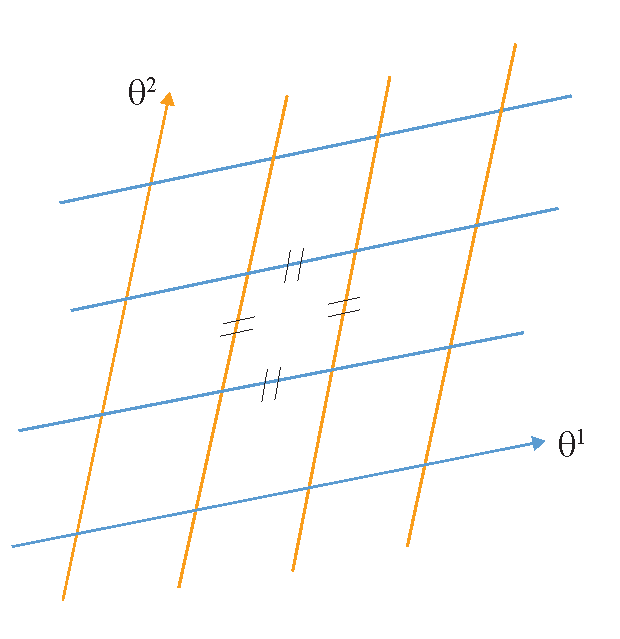
\includegraphics[width=0.6\linewidth ]{figure/Theory/equalMeshFrei.pdf}
\caption{The tangent differs depending of which direction you refer to. }
\end{figure}

This is a powerful concept working on for instance lattice structures such as gridshells where you can assign a constant length to the members.


\section{Form finding algorithms}

\subsection{Force Density}

\subsection{Thrust Network Analysis}

\begin{figure}[H]
\centering
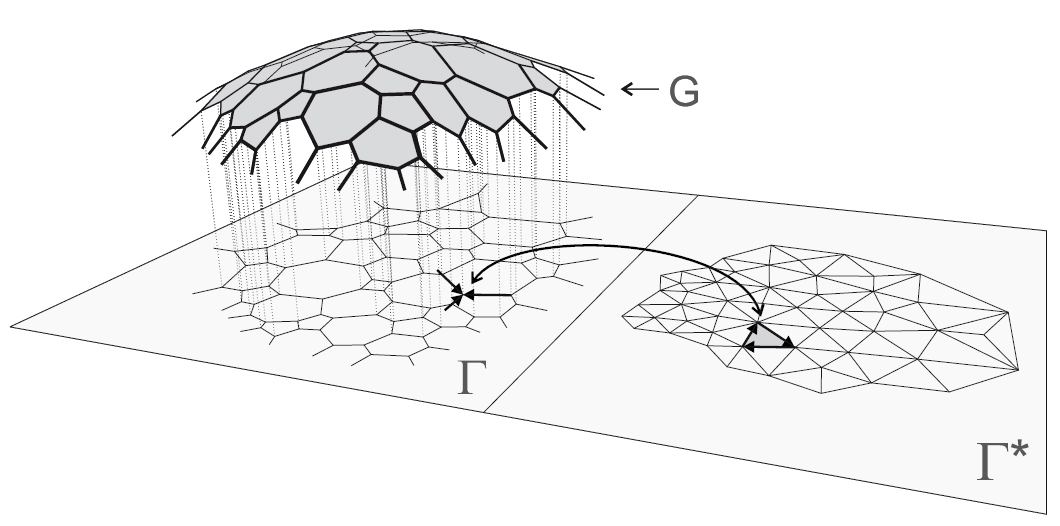
\includegraphics[width=0.6\linewidth ]{figure/Theory/TNA.jpg}
\caption{The tangent differs depending of which direction you refer to. }
\end{figure}

\begin{figure}[H]
\centering
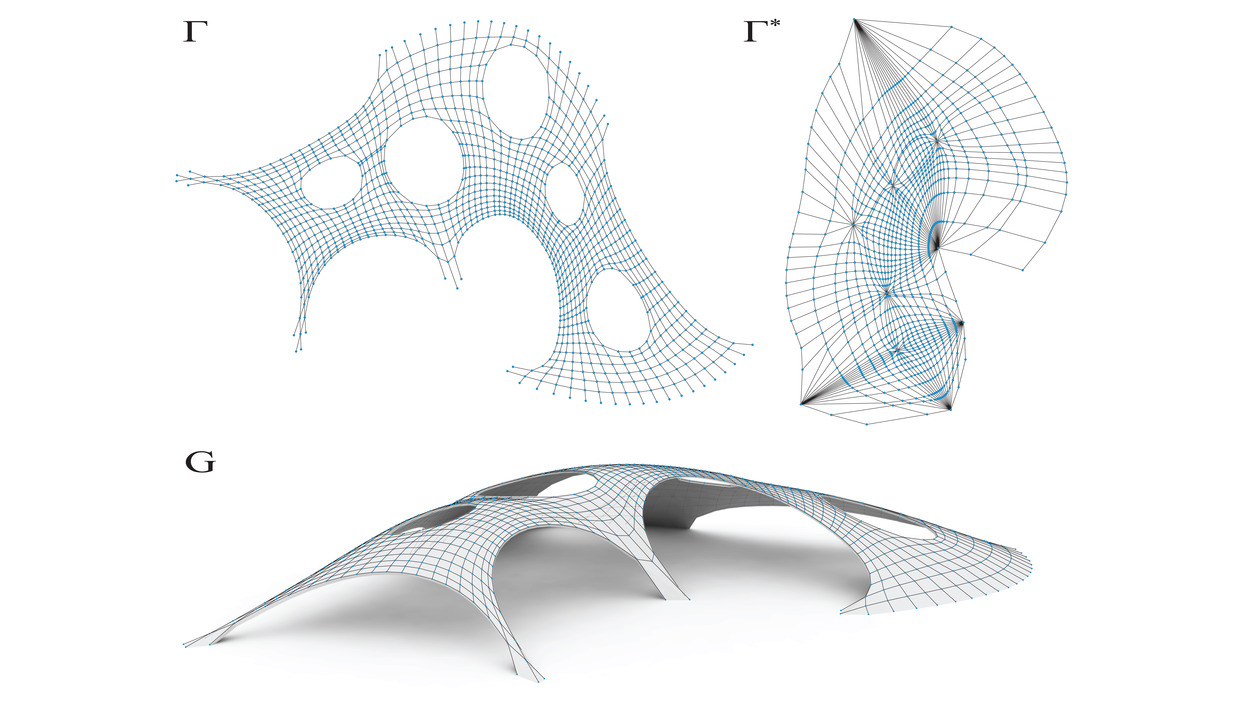
\includegraphics[width=0.6\linewidth ]{figure/Theory/RhinoVault.jpg}
\caption{The tangent differs depending of which direction you refer to. }
\end{figure}

\subsection{Dynamic Relaxation}

The basic equation of dynamics is based on Newtons second law of motion. So the sum of all forces in the system is equal to the mass times acceleration.

\begin{equation}
\sum F = ma
\end{equation}

"Dynamic Relaxation was invented by \textit{ Alistar Day} in 1965 and is a numerical procedure that solves a set of nonlinear equations. Summarized, the technique traces the motion of the structure through time under applied load. The technique is effectively the same as the leapfrog and Verlet methods, which are also used to integrate Newton's second law through time.\\
The basis of the method is to trace the step by step for small time increments, $\Delta t$, the motion of each interconnected node of the grid until the structure comes to rest in static equilibrium."

A typical flow diagram of dynamic relaxation can look like this. It is a modified version of one from Shell structures for architecture. That one is made for modelling a grid-shell so this one is a bit more general:

\begin{figure}[H]
\centering
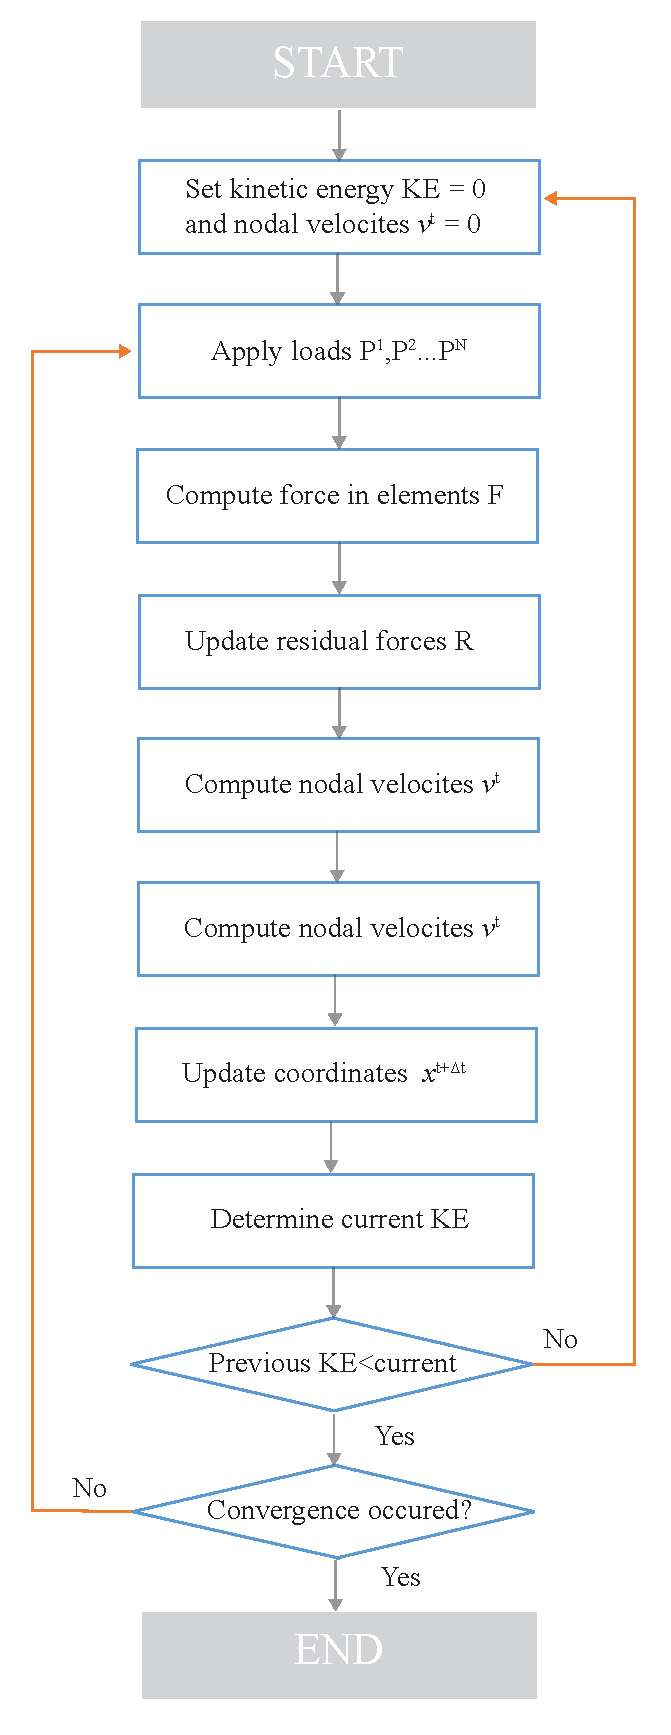
\includegraphics[height=1.2\linewidth ]{figure/Theory/DRScheme.pdf}
\caption{Flow diagram for Dynamic Relaxation }
\end{figure}

It has been commonly used in engineering to find forms of equilibrium for membrane and shell structures. For the former the DR formulation is very dependent of the internal forces and the pretension its elements or boundaries. Shells on the other hand is very dependent of the external loads and has a dominant gravity force applied.Though you can really model any kind of loading as long it imposes a force on the nodes or particles.

\subsubsection{Combined form-finding and cutting patterns of tensile structures}

Form finding a fabric structure with a soap film or minimal surface is done by setting the membrane stress components:

\begin{equation}
    n^{\alpha \beta} = Ta^{\alpha \beta}
\end{equation}

$T$ is the surface tension and $a^{\alpha \beta}$ is the metric tensor. In addition a geodesic coordinate system for generating the cutting pattern is obtained by imposing the conditions $a^{12} = 0$ and  $a^{22} = constant$


\begin{figure}[H]
\centering
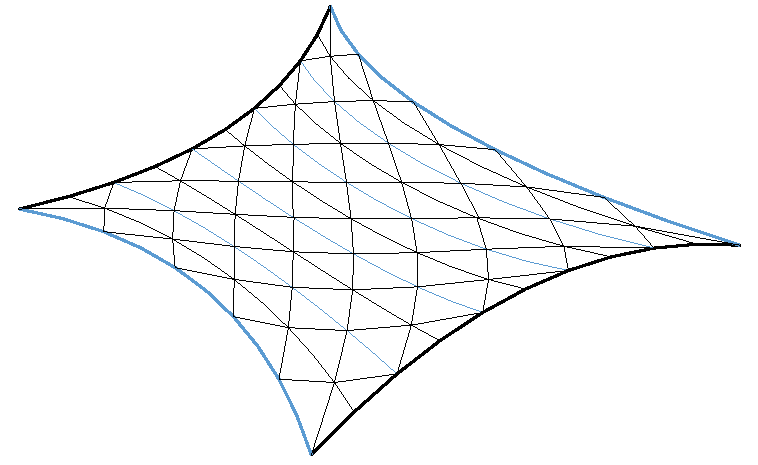
\includegraphics[width=0.9\linewidth ]{figure/Theory/EqualMeshGeo.pdf}
\caption{Flow diagram for Dynamic Relaxation }
\end{figure}


\begin{figure}[H]
\centering
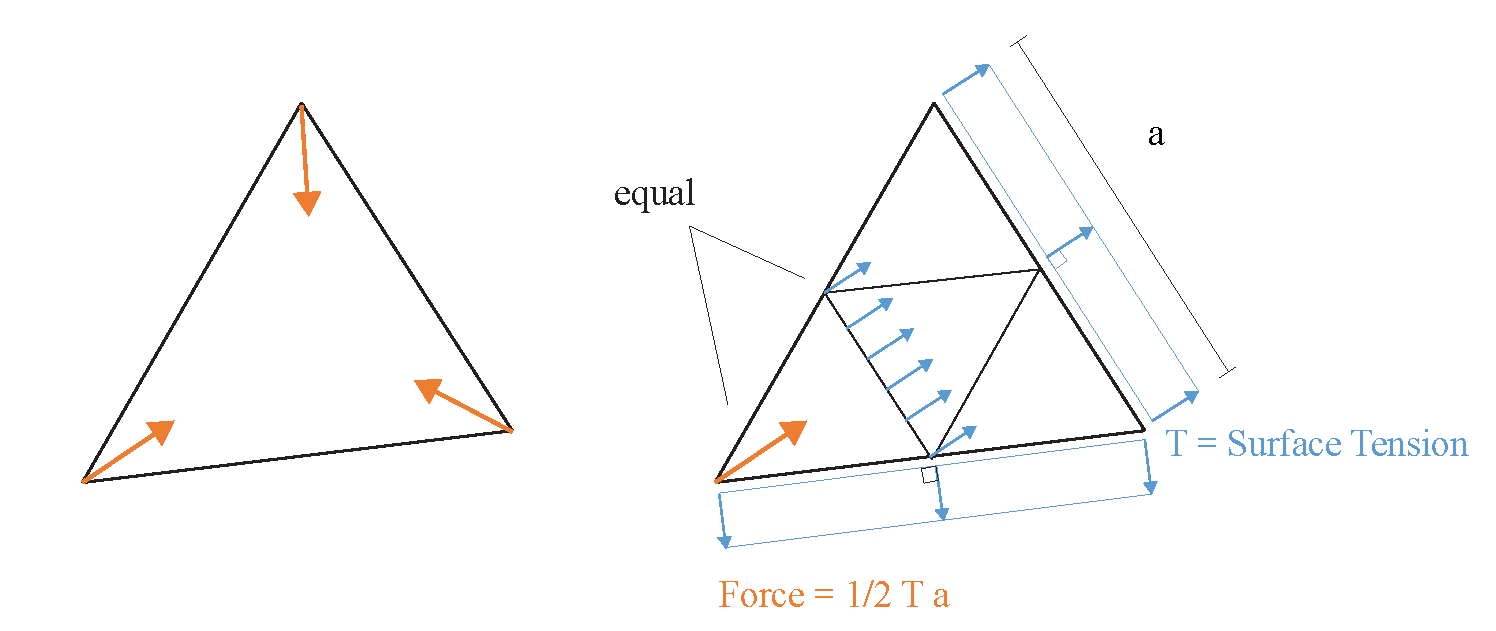
\includegraphics[width=1.0\linewidth ]{figure/Theory/SoapbubbleElement.pdf}
\caption{Flow diagram for Dynamic Relaxation }
\end{figure}


\section{Shell Theory}




\subsection{Curved beams}

Before heading into the membrane theory of shells we can look at an curved beam element.

\begin{figure}[H]
\centering
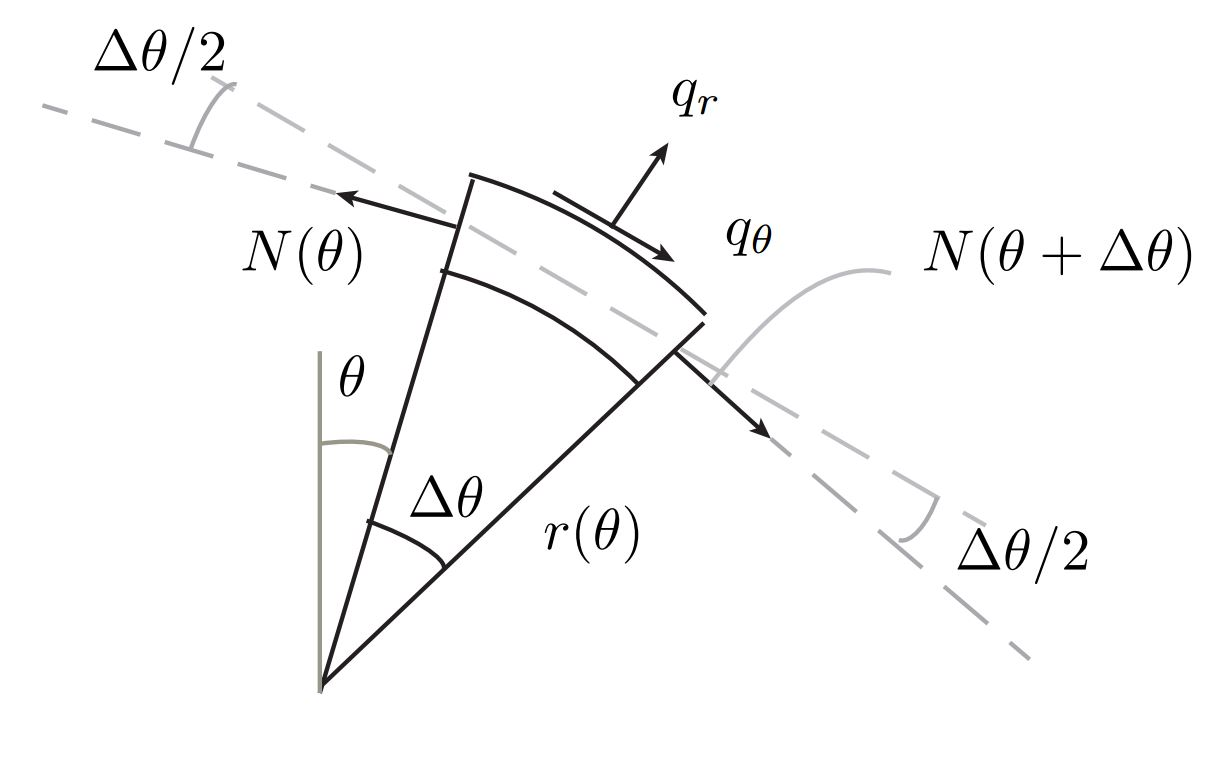
\includegraphics[height=0.5\linewidth ]{figure/Theory/CurvedBeam.JPG}
\caption{The tangent differs depending of which direction you refer to. }
\end{figure}
\subsection{General Theory of Membrane Shells}


Shells, in which bending moments can be neglected are called membrane
shells. Membrane theory assumes the following things:

\begin{itemize}
\item The material of the shell is isotropic and obeys Hooke's law.
\item The thickness of the shell (and the bending moments) can be neglected.
\item The state of stress of the shell is fully described by the membrane
forces acting in the mean surface.
\item Supports along the boundary are tangent to the mean surface.
\item Deformations due to membrane forces are not hindered by boundary
conditions.
\end{itemize}

\begin{figure}[H]
\centering
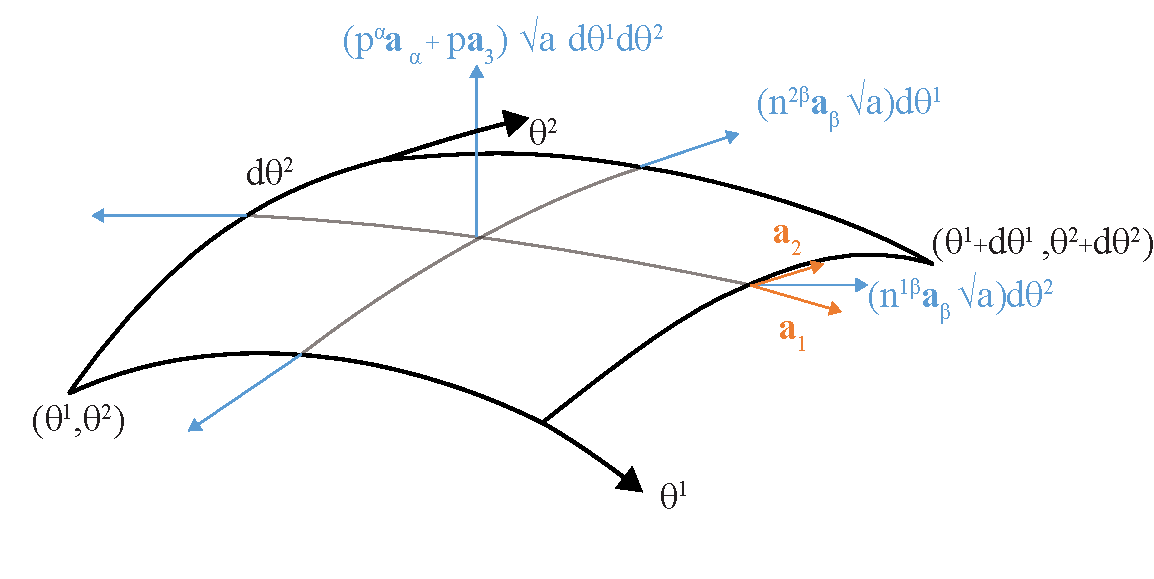
\includegraphics[width=0.9\linewidth ]{figure/Theory/membraneDefinition.pdf}
\caption{The tangent differs depending of which direction you refer to. }
\end{figure}


Equilibrium: 
\begin{equation}
\frac{\partial}{\partial \theta^1}(n^{1 \beta}\textbf{a}_{\beta} \sqrt{a}) d\theta^2 d\theta^1 + \frac{\partial}{\partial \theta^2}(n^{2 \beta}\textbf{a}_{\beta} \sqrt{a}) d\theta^1 d\theta^2 + ( p^{\alpha}\textbf{a}_\alpha + p\textbf{a}_3)\sqrt{a} d\theta^1 d\theta^2  = 0
\end{equation}



\begin{equation} \label{membraneEq}
\therefore  \frac{\partial}{\partial \theta^ \alpha} (n^{\alpha \beta} \textbf{a}_\beta \sqrt{ a}) + ( p^{\alpha}\textbf{a}_\alpha + p\textbf{a}_3)\sqrt{a} = 0
\end{equation}

Vector 3 equations

From \ref{membraneEq}

\begin{equation}
n^{\alpha \beta}_{,\alpha} \textbf{a}_\beta + n^{\alpha \beta}\textbf{a}_{\beta,\alpha} + n^{\alpha \beta}\textbf{a}_\beta \Gamma^\lambda_{\lambda \alpha} + (p^\beta \textbf{a}_\beta + p\textbf{a}_3) = 0
\end{equation}

Coefficients of $\textbf{a}_\beta$,  2 equations.
\begin{equation}
(n^{\alpha \beta}_{,\alpha} + n^{\alpha \beta}\Gamma^\beta_{\lambda \alpha} + n^{\alpha \beta}\Gamma^\lambda_{\lambda \alpha} + p^\beta) \textbf{a}_\beta = 0 
\end{equation}

Coefficients of $\textbf{a}_3$,  1 equation.
\begin{equation}
(n^{\alpha \beta} b_{\alpha \beta} + p)\textbf{a}_3 = 0
\end{equation}

The shell is subjected to external loads which is dentoted by $\textbf{p}$ and is measured per unit area of the middle surface.

\begin{equation}
\textbf{p} = p^{\alpha}\textbf{a}_\alpha +p\textbf{a}_3
\end{equation}


Equilibrium equations:
\begin{equation}
n^{\alpha \beta}b_{\alpha \beta} + p = 0
\end{equation}
\begin{equation}
n^{\alpha \beta}|_\alpha + p^\beta = 0
\end{equation}

Where $n^{\alpha \beta}|_\alpha$ is the covariant differentiation. 

\begin{equation}
n^{\alpha \beta}|_\alpha = n^{\alpha \beta}_{,a} + \Gamma^\beta_{\alpha \rho} n^{\alpha \rho} + \Gamma^\alpha_{\alpha \rho} n^{\rho \beta}
\end{equation}


\begin{figure}[H]
\centering
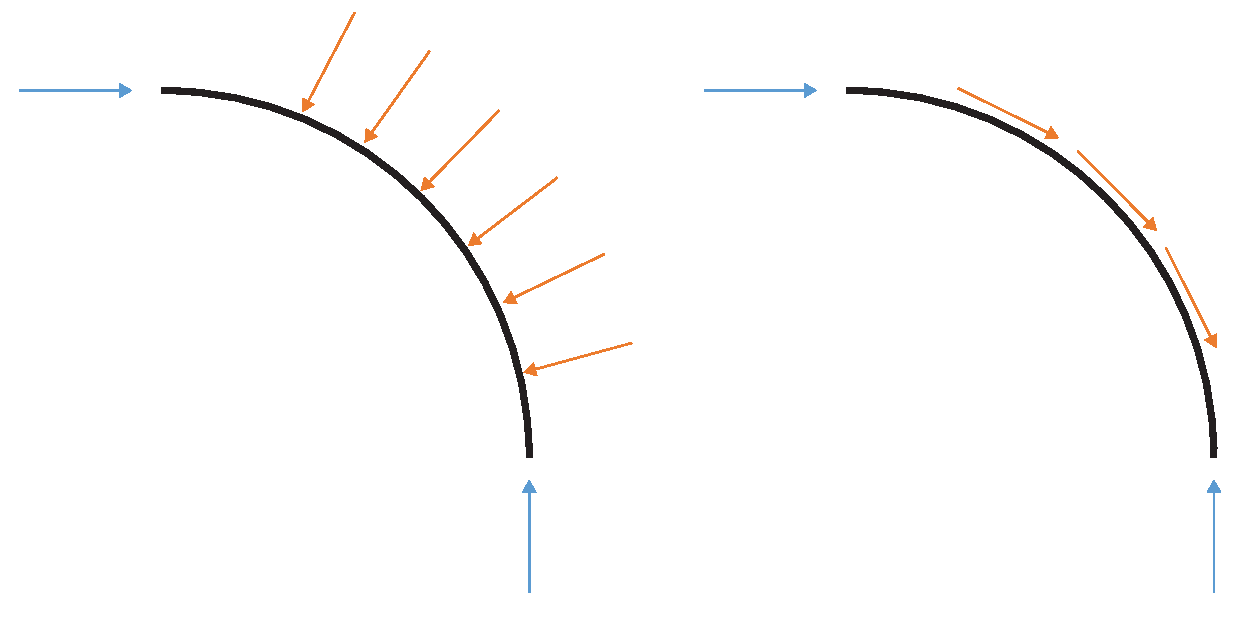
\includegraphics[width=0.9\linewidth ]{figure/Theory/equlibriumMem.pdf}
\caption{The tangent differs depending of which direction you refer to. }
\end{figure}

\subsection{Membrane Theory In Plane Coordinates}
It is sometimes useful to have the membrane theory expressed in a base plane $\Pi$. This is for instance a vital part of the \textit{Thrust network analysis} method presented in \textit{Philippe Blocks} Phd.

"We consider a net of coordinate curves on the middle surface M and we form a parallel projection on this net on to a plane $\Pi$. The direction of the projection is given by the unit vector $\textbf{e}_3$ which is perpendicular to $\Pi$ and measured from $\Pi$ to $M$. We now have a net od coordinate curves on $\Pi$ which corresponds to the net of $M$ and we assume that correspondence is one-one. The distance between two corresponding points of  $M$ and $\Pi$ is measured in the direction of $\textbf{e}_3$ is denoted by $z(\theta^1, \theta^2)$ which is a function of $\theta^1,\theta^2$ and us a surface invariant.Taking the \textbf{r} for the position vector of $M$, and $\hat{\textbf{r}}$ for the position vector of the corresponding point of $\Pi$, we have $\textbf{r} = \hat{\textbf{r}} + z \textbf{e}_3$."

\begin{figure}[H]
\centering
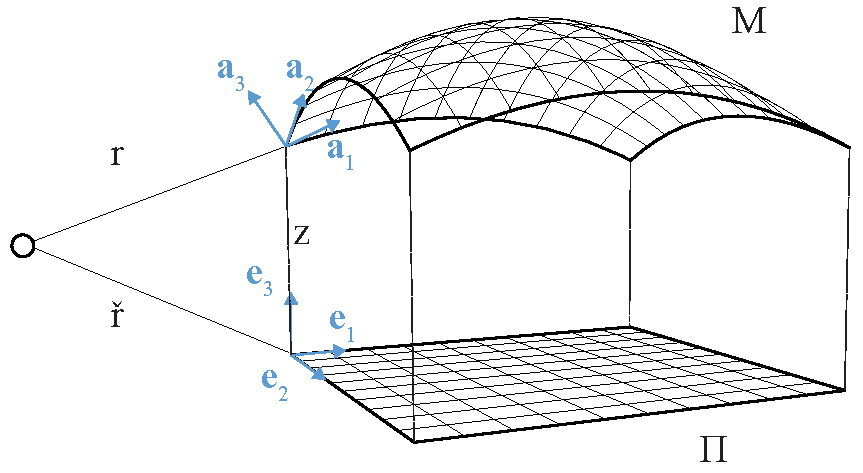
\includegraphics[width=0.9\linewidth ]{figure/Theory/planeShell.pdf}
\caption{Drawn from Zerna }
\end{figure}


\begin{equation}\label{memEq}
\epsilon^{\alpha \gamma}\epsilon^{\beta \rho} z|_{\alpha \beta}\phi|_{\gamma \rho} = q
\end{equation}
Where q contains the loading acting on the shell. 
\begin{equation}
q = z|_{\alpha \beta}A^{\alpha \beta} - s + s^\alpha z |_\alpha
\end{equation}

If writing out these equation \ref{memEq} we get 16 equations since we have four summation indices. Zerna define the components of the  psuedo-Tensor as $\epsilon^{11} = \epsilon^{22}=\epsilon_{11}=\epsilon_{22} = 0,\quad \epsilon^{12} = -\epsilon^{21} = \sqrt{a},\quad \epsilon_{12} = -\epsilon_{21} = \frac{1}{\sqrt{a}},$ It is possible to reduce it to:

\begin{equation}
    \epsilon^{21}\epsilon^{21}z,_{22}\phi_{11} + 2\epsilon^{12}\epsilon^{21}z,_{12}\phi_{12} + \epsilon^{12}\epsilon^{12}z,_{11}\phi_{22} = q
\end{equation}

If we choose a rectangular Cartesian coordinate system we can simplify the expression to:

\begin{equation}
    z,_{22}\phi_{11} -2 z,_{12}\phi_{12} + z,_{11}\phi_{22} = q
\end{equation}

This is the equation you can read in books the famous book \textit{Theory of Plates and Shells} by Timoshenko and Woinowsky-Krieger for membrane stresses in shells. They use and \textit{F} instead of $\phi$ for stress functions.

\subsubsection{Airy Stress Functions}

    
\begin{equation}
\sigma_x = \frac{\partial^2\phi}{\partial y^2}, \sigma_y = \frac{\partial^2\phi}{\partial x^2}, \sigma_{xy} = \frac{\partial^2\phi}{\partial x \partial y}
\end{equation}

